% **************************************************************************************************************
% A Classic Thesis Style
% An Homage to The Elements of Typographic Style
%
% Copyright (C) 2017 André Miede and Ivo Pletikosić
%
% If you like the style then I would appreciate a postcard. My address
% can be found in the file ClassicThesis.pdf. A collection of the
% postcards I received so far is available online at
% http://postcards.miede.de
%
% License:
% This program is free software; you can redistribute it and/or modify
% it under the terms of the GNU General Public License as published by
% the Free Software Foundation; either version 2 of the License, or
% (at your option) any later version.
%
% This program is distributed in the hope that it will be useful,
% but WITHOUT ANY WARRANTY; without even the implied warranty of
% MERCHANTABILITY or FITNESS FOR A PARTICULAR PURPOSE.  See the
% GNU General Public License for more details.
%
% You should have received a copy of the GNU General Public License
% along with this program; see the file COPYING.  If not, write to
% the Free Software Foundation, Inc., 59 Temple Place - Suite 330,
% Boston, MA 02111-1307, USA.
%
% PLEASE THE ALSO THE AUTHORS' NOTE REGARDING THIS LICENCSE
% IN THE DOCUMENTATION (ClassicThesis.pdf --> Chapter 1 / Chapter01.tex)
% **************************************************************************************************************
\RequirePackage{silence} % :-\
    \WarningFilter{scrreprt}{Usage of package `titlesec'}
    %\WarningFilter{scrreprt}{Activating an ugly workaround}
    \WarningFilter{titlesec}{Non standard sectioning command detected}
\RequirePackage{fix-cm} % fix some latex issues see: http://texdoc.net/texmf-dist/doc/latex/base/fixltx2e.pdf
\documentclass[ twoside,openright,titlepage,numbers=noenddot,headinclude,%1headlines,% letterpaper a4paper
                footinclude=true,cleardoublepage=empty,abstractoff, % <--- obsolete, remove (todo)
                BCOR=5mm,paper=a4,fontsize=11pt,%11pt,a4paper,%
                ngerman,american,%
                ]{scrreprt}

%********************************************************************
% Note: Make all your adjustments in here
%*******************************************************
% ****************************************************************************************************
% classicthesis-config.tex
% formerly known as loadpackages.sty, classicthesis-ldpkg.sty, and classicthesis-preamble.sty
% Use it at the beginning of your ClassicThesis.tex, or as a LaTeX Preamble
% in your ClassicThesis.{tex,lyx} with % ****************************************************************************************************
% classicthesis-config.tex
% formerly known as loadpackages.sty, classicthesis-ldpkg.sty, and classicthesis-preamble.sty
% Use it at the beginning of your ClassicThesis.tex, or as a LaTeX Preamble
% in your ClassicThesis.{tex,lyx} with % ****************************************************************************************************
% classicthesis-config.tex
% formerly known as loadpackages.sty, classicthesis-ldpkg.sty, and classicthesis-preamble.sty
% Use it at the beginning of your ClassicThesis.tex, or as a LaTeX Preamble
% in your ClassicThesis.{tex,lyx} with \input{classicthesis-config}
% ****************************************************************************************************
% If you like the classicthesis, then I would appreciate a postcard.
% My address can be found in the file ClassicThesis.pdf. A collection
% of the postcards I received so far is available online at
% http://postcards.miede.de
% ****************************************************************************************************


% ****************************************************************************************************
% 0. Set the encoding of your files. UTF-8 is the only sensible encoding nowadays. If you can't read
% äöüßáéçèê∂åëæƒÏ€ then change the encoding setting in your editor, not the line below. If your editor
% does not support utf8 use another editor!
% ****************************************************************************************************
\PassOptionsToPackage{utf8}{inputenc}
  \usepackage{inputenc}

\PassOptionsToPackage{T1}{fontenc} % T2A for cyrillics
  \usepackage{fontenc}


% ****************************************************************************************************
% 1. Configure classicthesis for your needs here, e.g., remove "drafting" below
% in order to deactivate the time-stamp on the pages
% (see ClassicThesis.pdf for more information):
% ****************************************************************************************************
\PassOptionsToPackage{
  drafting=false,    % print version information on the bottom of the pages
  tocaligned=false, % the left column of the toc will be aligned (no indentation)
  dottedtoc=false,  % page numbers in ToC flushed right
  eulerchapternumbers=true, % use AMS Euler for chapter font (otherwise Palatino)
  linedheaders=false,       % chaper headers will have line above and beneath
  floatperchapter=true,     % numbering per chapter for all floats (i.e., Figure 1.1)
  eulermath=false,  % use awesome Euler fonts for mathematical formulae (only with pdfLaTeX)
  beramono=true,    % toggle a nice monospaced font (w/ bold)
  palatino=true,    % deactivate standard font for loading another one, see the last section at the end of this file for suggestions
  style=arsclassica % classicthesis, arsclassica
}{classicthesis}


% ****************************************************************************************************
% 2. Personal data and user ad-hoc commands (insert your own data here)
% ****************************************************************************************************
\input{revision}

% Separation and Count Estimation for Audio Signals Overlapping in Time and Frequency
% Trennung und Schätzung der Anzahl von Zeit- und Frequenzüberlappenden Audiosignalen

\newcommand{\myTitle}{Separation and Count Estimation for Audio Sources Overlapping in Time and Frequency\xspace}
\newcommand{\myTitleGerman}{Trennung und Schätzung der Anzahl von Audiosignalquellen mit Zeit- und Frequenzüberlappung\xspace}
\newcommand{\mySubtitle}{test\xspace}
\newcommand{\myDegree}{Doktor-Ingenieur (Dr.-Ing.)\xspace}
\newcommand{\myName}{Fabian-Robert Stöter\xspace}
\newcommand{\myProf}{Prof. Dr.-Ing. Bernd Edler\xspace}
\newcommand{\myOtherProf}{Prof. Gaël Richard (Ph.D)\xspace}
\newcommand{\mySupervisor}{Put name here\xspace}
\newcommand{\myFaculty}{International Audio Laboratories Erlangen\xspace}
\newcommand{\myDepartment}{\xspace}
\newcommand{\myUni}{Universität Erlangen-Nürnberg\xspace}
\newcommand{\myLocation}{Montpellier\xspace}
\newcommand{\myTime}{7. April 2019\xspace}
\newcommand{\myVersion}{commit \revision}

% ********************************************************************
% Setup, finetuning, and useful commands
% ********************************************************************
\providecommand{\mLyX}{L\kern-.1667em\lower.25em\hbox{Y}\kern-.125emX\@}
\newcommand{\ie}{i.\,e.}
\newcommand{\Ie}{I.\,e.}
\newcommand{\eg}{e.\,g.}
\newcommand{\Eg}{E.\,g.}
% ****************************************************************************************************


% ****************************************************************************************************
% 3. Loading some handy packages
% ****************************************************************************************************
% ********************************************************************
% Packages with options that might require adjustments
% ********************************************************************
\PassOptionsToPackage{ngerman,american}{babel} % change this to your language(s), main language last
% Spanish languages need extra options in order to work with this template
%\PassOptionsToPackage{spanish,es-lcroman}{babel}
    \usepackage{babel}

\usepackage{csquotes}

\PassOptionsToPackage{%
  backend=biber,bibencoding=utf8, %instead of bibtex
  % backend=bibtex8,bibencoding=ascii,%
  language=auto,%
  % style=ieee,%
  % dashed=false,
  firstinits=true,
  defernumbers,
  style=ieee, % Author 1999, 2010
  citestyle=numeric-comp,
  dashed=false,
  %bibstyle=authoryear,dashed=false, % dashed: substitute rep. author with ---
  sorting=nyt, % name, year, title
  maxbibnames=10, % default: 3, et al.
  %backref=true,%
  natbib=false % natbib compatibility mode (\citep and \citet still work)
}{biblatex}

\usepackage{biblatex}


% Emphasize own name in References with boldface
\usepackage{xpatch}

\usepackage{float}
\usepackage{amsmath,amssymb,amsfonts,amsthm,bm}
\usepackage{euscript}

%----------------------
\usepackage{tikz}
\usetikzlibrary{positioning,fit, calc}
\usepackage{pgfplots}

\usepackage{bm}

% ********************************************************************
% General useful packages
% ********************************************************************
\usepackage{graphicx} %
\usepackage{float}
\usepackage{scrhack} % fix warnings when using KOMA with listings package
\usepackage{xspace} % to get the spacing after macros right
\PassOptionsToPackage{printonlyused,smaller}{acronym}
  \usepackage{acronym} % nice macros for handling all acronyms in the thesis
  %\renewcommand{\bflabel}[1]{{#1}\hfill} % fix the list of acronyms --> no longer working
  %\renewcommand*{\acsfont}[1]{\textsc{#1}}
  %\renewcommand*{\aclabelfont}[1]{\acsfont{#1}}
  %\def\bflabel#1{{#1\hfill}}
  \def\bflabel#1{{\acsfont{#1}\hfill}}
  \def\aclabelfont#1{\acsfont{#1}}
% ****************************************************************************************************
\usepackage{pgfplots} % External TikZ/PGF support (thanks to Andreas Nautsch)
% \usetikzlibrary{external}
% \tikzexternalize[mode=list and make, prefix=ext-tikz/]
% ****************************************************************************************************


% ****************************************************************************************************
% 4. Setup floats: tables, (sub)figures, and captions
% ****************************************************************************************************
\usepackage{tabularx} % better tables
  \setlength{\extrarowheight}{3pt} % increase table row height
\newcommand{\tableheadline}[1]{\multicolumn{1}{l}{\spacedlowsmallcaps{#1}}}
\newcommand{\myfloatalign}{\centering} % to be used with each float for alignment

% ****************************************************************************************************

% ****************************************************************************************************
% 5. Setup code listings
% ****************************************************************************************************
% \usepackage{listings}
\usepackage{longtable}

%\lstset{emph={trueIndex,root},emphstyle=\color{BlueViolet}}%\underbar} % for special keywords
% \lstset{language=[LaTeX]Tex,%C++,
%   morekeywords={PassOptionsToPackage,selectlanguage},
%   keywordstyle=\color{RoyalBlue},%\bfseries,
%   basicstyle=\small\ttfamily,
%   %identifierstyle=\color{NavyBlue},
%   commentstyle=\color{Green}\ttfamily,
%   stringstyle=\rmfamily,
%   numbers=none,%left,%
%   numberstyle=\scriptsize,%\tiny
%   stepnumber=5,
%   numbersep=8pt,
%   showstringspaces=false,
%   breaklines=true,
%   %frameround=ftff,
%   %frame=single,
%   belowcaptionskip=.75\baselineskip
%   %frame=L
% }
% ****************************************************************************************************
\usepackage{setspace}
\usepackage[newfloat]{minted}
\usemintedstyle{tango}
\definecolor{tango-bg}{HTML}{F8F8F8}

\newminted{python}{bgcolor=tango-bg,frame=lines,framesep=2mm,samepage=true,fontsize=\footnotesize}


% ****************************************************************************************************
% 6. Last calls before the bar closes
% ****************************************************************************************************
% ********************************************************************
% Her Majesty herself
% ********************************************************************
\usepackage{classicthesis}


% ********************************************************************
% Fine-tune hyperreferences (hyperref should be called last)
% ********************************************************************
\hypersetup{%
  %draft, % hyperref's draft mode, for printing see below
  % colorlinks=true, linktocpage=true, pdfstartpage=3, pdfstartview=FitV,%
  % uncomment the following line if you want to have black links (e.g., for printing)
  colorlinks=true, linktocpage=false, pdfstartpage=3, pdfstartview=FitV, pdfborder={0 0 0},%
  breaklinks=true, pageanchor=true,%
  pdfpagemode=UseNone, %
  % pdfpagemode=UseOutlines,%
  plainpages=false, bookmarksnumbered, bookmarksopen=true, bookmarksopenlevel=1,%
  hypertexnames=true, pdfhighlight=/O,%nesting=true,%frenchlinks,%
  urlcolor=CTurl, linkcolor=CTlink, citecolor=CTcitation, %pagecolor=RoyalBlue,%
  %urlcolor=Black, linkcolor=Black, citecolor=Black, %pagecolor=Black,%
  pdftitle={\myTitle},%
  pdfauthor={\textcopyright\ \myName, \myUni, \myFaculty},%
  pdfsubject={},%
  pdfkeywords={},%
  pdfcreator={pdfLaTeX},%
  pdfproducer={LaTeX with hyperref and classicthesis}%
}


% ********************************************************************
% Setup autoreferences (hyperref and babel)
% ********************************************************************
% There are some issues regarding autorefnames
% http://www.tex.ac.uk/cgi-bin/texfaq2html?label=latexwords
% you have to redefine the macros for the
% language you use, e.g., american, ngerman
% (as chosen when loading babel/AtBeginDocument)
% ********************************************************************
\makeatletter
\@ifpackageloaded{babel}%
  {%
    \addto\extrasamerican{%
      \renewcommand*{\figureautorefname}{Figure}%
      \renewcommand*{\tableautorefname}{Table}%
      \renewcommand*{\partautorefname}{Part}%
      \renewcommand*{\chapterautorefname}{Chapter}%
      \renewcommand*{\sectionautorefname}{Section}%
      \renewcommand*{\subsectionautorefname}{Section}%
      \renewcommand*{\subsubsectionautorefname}{Section}%
    }%
    \addto\extrasngerman{%
      \renewcommand*{\paragraphautorefname}{Absatz}%
      \renewcommand*{\subparagraphautorefname}{Unterabsatz}%
      \renewcommand*{\footnoteautorefname}{Fu\"snote}%
      \renewcommand*{\FancyVerbLineautorefname}{Zeile}%
      \renewcommand*{\theoremautorefname}{Theorem}%
      \renewcommand*{\appendixautorefname}{Anhang}%
      \renewcommand*{\equationautorefname}{Gleichung}%
      \renewcommand*{\itemautorefname}{Punkt}%
    }%
      % Fix to getting autorefs for subfigures right (thanks to Belinda Vogt for changing the definition)
      \providecommand{\subfigureautorefname}{\figureautorefname}%
    }{\relax}
\makeatother


% ********************************************************************
% Development Stuff
% ********************************************************************
\listfiles
%\PassOptionsToPackage{l2tabu,orthodox,abort}{nag}
%  \usepackage{nag}
%\PassOptionsToPackage{warning, all}{onlyamsmath}
%  \usepackage{onlyamsmath}


% ****************************************************************************************************
% 7. Further adjustments (experimental)
% ****************************************************************************************************
% ********************************************************************
% Changing the text area
% ********************************************************************
%\areaset[current]{312pt}{761pt} % 686 (factor 2.2) + 33 head + 42 head \the\footskip
%\setlength{\marginparwidth}{7em}%
%\setlength{\marginparsep}{2em}%

% ********************************************************************
% Using different fonts
% ********************************************************************
%\usepackage[oldstylenums]{kpfonts} % oldstyle notextcomp
% \usepackage[osf]{libertine}
%\usepackage[light,condensed,math]{iwona}
%\renewcommand{\sfdefault}{iwona}
%\usepackage{lmodern} % <-- no osf support :-(
%\usepackage{cfr-lm} %
%\usepackage[urw-garamond]{mathdesign} <-- no osf support :-(
%\usepackage[default,osfigures]{opensans} % scale=0.95
% \usepackage[sfdefault]{FiraSans}
% \usepackage[opticals,mathlf]{MinionPro} % onlytext
% ********************************************************************
%\usepackage[largesc,osf]{newpxtext}
%\linespread{1.05} % a bit more for Palatino
% Used to fix these:
% https://bitbucket.org/amiede/classicthesis/issues/139/italics-in-pallatino-capitals-chapter
% https://bitbucket.org/amiede/classicthesis/issues/45/problema-testatine-su-classicthesis-style
% ********************************************************************
% ****************************************************************************************************

\newcommand{\contribs}[1]{
  \begin{minipage}{.3\linewidth}
  \end{minipage}
  \hfill
  \begin{minipage}{.67\linewidth}
    %\begin{flushright}
      \begin{small}
        \textcolor{gray}{\textsf{#1}}
      \end{small}
      \vspace{20pt}\\
    %\end{flushright}
  \end{minipage}
}

\input{mathcommands.tex}

\usepackage{siunitx}

\floatstyle{ruled}
\newfloat{algorithm}{tbp}{loa}
\providecommand{\algorithmname}{Algorithm}
\floatname{algorithm}{\protect\algorithmname}

% Example definitions.
\def\x{{\mathbf{x}}}
\def\L{{\cal{L}}}
\def\Pitch{{F}}

% Official addiontional AudioLabs colors
\definecolor{nice}{rgb}{0.8,0.725490196078431,0.454901960784314}
\definecolor{almagenta}{RGB}{210,85,255}
\definecolor{alturquise}{RGB}{43,174,91}
\definecolor{algreen}{RGB}{111,217,0}
\definecolor{alturquisedark}{RGB}{0,151,164}

% Example definitions.
% --------------------
\providecommand{\e}[1]{\ensuremath{\times 10^{#1}}}


% \renewcommand\formatchapter[1]{%
%     \setbox0=\hbox{\chapterNumber\thechapter\hspace{10pt}\vline\ }%
%     \begin{minipage}[t]{\dimexpr\linewidth-\wd0\relax}%
%     \raggedright\spacedallcaps{#1}%
%     \end{minipage}%
% }

\usepackage{caption}

\newenvironment{code}{\captionsetup{type=listing}}{}
\SetupFloatingEnvironment{listing}{name=Source Code}

\usepackage{framed} 
\definecolor{shadecolor}{gray}{0.9} 

\hyphenation{Sou-mi-tro}
\hyphenation{Cha-kra-bar-ty}

% ****************************************************************************************************
% If you like the classicthesis, then I would appreciate a postcard.
% My address can be found in the file ClassicThesis.pdf. A collection
% of the postcards I received so far is available online at
% http://postcards.miede.de
% ****************************************************************************************************


% ****************************************************************************************************
% 0. Set the encoding of your files. UTF-8 is the only sensible encoding nowadays. If you can't read
% äöüßáéçèê∂åëæƒÏ€ then change the encoding setting in your editor, not the line below. If your editor
% does not support utf8 use another editor!
% ****************************************************************************************************
\PassOptionsToPackage{utf8}{inputenc}
  \usepackage{inputenc}

\PassOptionsToPackage{T1}{fontenc} % T2A for cyrillics
  \usepackage{fontenc}


% ****************************************************************************************************
% 1. Configure classicthesis for your needs here, e.g., remove "drafting" below
% in order to deactivate the time-stamp on the pages
% (see ClassicThesis.pdf for more information):
% ****************************************************************************************************
\PassOptionsToPackage{
  drafting=false,    % print version information on the bottom of the pages
  tocaligned=false, % the left column of the toc will be aligned (no indentation)
  dottedtoc=false,  % page numbers in ToC flushed right
  eulerchapternumbers=true, % use AMS Euler for chapter font (otherwise Palatino)
  linedheaders=false,       % chaper headers will have line above and beneath
  floatperchapter=true,     % numbering per chapter for all floats (i.e., Figure 1.1)
  eulermath=false,  % use awesome Euler fonts for mathematical formulae (only with pdfLaTeX)
  beramono=true,    % toggle a nice monospaced font (w/ bold)
  palatino=true,    % deactivate standard font for loading another one, see the last section at the end of this file for suggestions
  style=arsclassica % classicthesis, arsclassica
}{classicthesis}


% ****************************************************************************************************
% 2. Personal data and user ad-hoc commands (insert your own data here)
% ****************************************************************************************************
% Autogenerated, do not edit
\newcommand{\revisiondate}{2018-10-12}
\newcommand{\revision}{134f96f}


% Separation and Count Estimation for Audio Signals Overlapping in Time and Frequency
% Trennung und Schätzung der Anzahl von Zeit- und Frequenzüberlappenden Audiosignalen

\newcommand{\myTitle}{Separation and Count Estimation for Audio Sources Overlapping in Time and Frequency\xspace}
\newcommand{\myTitleGerman}{Trennung und Schätzung der Anzahl von Audiosignalquellen mit Zeit- und Frequenzüberlappung\xspace}
\newcommand{\mySubtitle}{test\xspace}
\newcommand{\myDegree}{Doktor-Ingenieur (Dr.-Ing.)\xspace}
\newcommand{\myName}{Fabian-Robert Stöter\xspace}
\newcommand{\myProf}{Prof. Dr.-Ing. Bernd Edler\xspace}
\newcommand{\myOtherProf}{Prof. Gaël Richard (Ph.D)\xspace}
\newcommand{\mySupervisor}{Put name here\xspace}
\newcommand{\myFaculty}{International Audio Laboratories Erlangen\xspace}
\newcommand{\myDepartment}{\xspace}
\newcommand{\myUni}{Universität Erlangen-Nürnberg\xspace}
\newcommand{\myLocation}{Montpellier\xspace}
\newcommand{\myTime}{7. April 2019\xspace}
\newcommand{\myVersion}{commit \revision}

% ********************************************************************
% Setup, finetuning, and useful commands
% ********************************************************************
\providecommand{\mLyX}{L\kern-.1667em\lower.25em\hbox{Y}\kern-.125emX\@}
\newcommand{\ie}{i.\,e.}
\newcommand{\Ie}{I.\,e.}
\newcommand{\eg}{e.\,g.}
\newcommand{\Eg}{E.\,g.}
% ****************************************************************************************************


% ****************************************************************************************************
% 3. Loading some handy packages
% ****************************************************************************************************
% ********************************************************************
% Packages with options that might require adjustments
% ********************************************************************
\PassOptionsToPackage{ngerman,american}{babel} % change this to your language(s), main language last
% Spanish languages need extra options in order to work with this template
%\PassOptionsToPackage{spanish,es-lcroman}{babel}
    \usepackage{babel}

\usepackage{csquotes}

\PassOptionsToPackage{%
  backend=biber,bibencoding=utf8, %instead of bibtex
  % backend=bibtex8,bibencoding=ascii,%
  language=auto,%
  % style=ieee,%
  % dashed=false,
  firstinits=true,
  defernumbers,
  style=ieee, % Author 1999, 2010
  citestyle=numeric-comp,
  dashed=false,
  %bibstyle=authoryear,dashed=false, % dashed: substitute rep. author with ---
  sorting=nyt, % name, year, title
  maxbibnames=10, % default: 3, et al.
  %backref=true,%
  natbib=false % natbib compatibility mode (\citep and \citet still work)
}{biblatex}

\usepackage{biblatex}


% Emphasize own name in References with boldface
\usepackage{xpatch}

\usepackage{float}
\usepackage{amsmath,amssymb,amsfonts,amsthm,bm}
\usepackage{euscript}

%----------------------
\usepackage{tikz}
\usetikzlibrary{positioning,fit, calc}
\usepackage{pgfplots}

\usepackage{bm}

% ********************************************************************
% General useful packages
% ********************************************************************
\usepackage{graphicx} %
\usepackage{float}
\usepackage{scrhack} % fix warnings when using KOMA with listings package
\usepackage{xspace} % to get the spacing after macros right
\PassOptionsToPackage{printonlyused,smaller}{acronym}
  \usepackage{acronym} % nice macros for handling all acronyms in the thesis
  %\renewcommand{\bflabel}[1]{{#1}\hfill} % fix the list of acronyms --> no longer working
  %\renewcommand*{\acsfont}[1]{\textsc{#1}}
  %\renewcommand*{\aclabelfont}[1]{\acsfont{#1}}
  %\def\bflabel#1{{#1\hfill}}
  \def\bflabel#1{{\acsfont{#1}\hfill}}
  \def\aclabelfont#1{\acsfont{#1}}
% ****************************************************************************************************
\usepackage{pgfplots} % External TikZ/PGF support (thanks to Andreas Nautsch)
% \usetikzlibrary{external}
% \tikzexternalize[mode=list and make, prefix=ext-tikz/]
% ****************************************************************************************************


% ****************************************************************************************************
% 4. Setup floats: tables, (sub)figures, and captions
% ****************************************************************************************************
\usepackage{tabularx} % better tables
  \setlength{\extrarowheight}{3pt} % increase table row height
\newcommand{\tableheadline}[1]{\multicolumn{1}{l}{\spacedlowsmallcaps{#1}}}
\newcommand{\myfloatalign}{\centering} % to be used with each float for alignment

% ****************************************************************************************************

% ****************************************************************************************************
% 5. Setup code listings
% ****************************************************************************************************
% \usepackage{listings}
\usepackage{longtable}

%\lstset{emph={trueIndex,root},emphstyle=\color{BlueViolet}}%\underbar} % for special keywords
% \lstset{language=[LaTeX]Tex,%C++,
%   morekeywords={PassOptionsToPackage,selectlanguage},
%   keywordstyle=\color{RoyalBlue},%\bfseries,
%   basicstyle=\small\ttfamily,
%   %identifierstyle=\color{NavyBlue},
%   commentstyle=\color{Green}\ttfamily,
%   stringstyle=\rmfamily,
%   numbers=none,%left,%
%   numberstyle=\scriptsize,%\tiny
%   stepnumber=5,
%   numbersep=8pt,
%   showstringspaces=false,
%   breaklines=true,
%   %frameround=ftff,
%   %frame=single,
%   belowcaptionskip=.75\baselineskip
%   %frame=L
% }
% ****************************************************************************************************
\usepackage{setspace}
\usepackage[newfloat]{minted}
\usemintedstyle{tango}
\definecolor{tango-bg}{HTML}{F8F8F8}

\newminted{python}{bgcolor=tango-bg,frame=lines,framesep=2mm,samepage=true,fontsize=\footnotesize}


% ****************************************************************************************************
% 6. Last calls before the bar closes
% ****************************************************************************************************
% ********************************************************************
% Her Majesty herself
% ********************************************************************
\usepackage{classicthesis}


% ********************************************************************
% Fine-tune hyperreferences (hyperref should be called last)
% ********************************************************************
\hypersetup{%
  %draft, % hyperref's draft mode, for printing see below
  % colorlinks=true, linktocpage=true, pdfstartpage=3, pdfstartview=FitV,%
  % uncomment the following line if you want to have black links (e.g., for printing)
  colorlinks=true, linktocpage=false, pdfstartpage=3, pdfstartview=FitV, pdfborder={0 0 0},%
  breaklinks=true, pageanchor=true,%
  pdfpagemode=UseNone, %
  % pdfpagemode=UseOutlines,%
  plainpages=false, bookmarksnumbered, bookmarksopen=true, bookmarksopenlevel=1,%
  hypertexnames=true, pdfhighlight=/O,%nesting=true,%frenchlinks,%
  urlcolor=CTurl, linkcolor=CTlink, citecolor=CTcitation, %pagecolor=RoyalBlue,%
  %urlcolor=Black, linkcolor=Black, citecolor=Black, %pagecolor=Black,%
  pdftitle={\myTitle},%
  pdfauthor={\textcopyright\ \myName, \myUni, \myFaculty},%
  pdfsubject={},%
  pdfkeywords={},%
  pdfcreator={pdfLaTeX},%
  pdfproducer={LaTeX with hyperref and classicthesis}%
}


% ********************************************************************
% Setup autoreferences (hyperref and babel)
% ********************************************************************
% There are some issues regarding autorefnames
% http://www.tex.ac.uk/cgi-bin/texfaq2html?label=latexwords
% you have to redefine the macros for the
% language you use, e.g., american, ngerman
% (as chosen when loading babel/AtBeginDocument)
% ********************************************************************
\makeatletter
\@ifpackageloaded{babel}%
  {%
    \addto\extrasamerican{%
      \renewcommand*{\figureautorefname}{Figure}%
      \renewcommand*{\tableautorefname}{Table}%
      \renewcommand*{\partautorefname}{Part}%
      \renewcommand*{\chapterautorefname}{Chapter}%
      \renewcommand*{\sectionautorefname}{Section}%
      \renewcommand*{\subsectionautorefname}{Section}%
      \renewcommand*{\subsubsectionautorefname}{Section}%
    }%
    \addto\extrasngerman{%
      \renewcommand*{\paragraphautorefname}{Absatz}%
      \renewcommand*{\subparagraphautorefname}{Unterabsatz}%
      \renewcommand*{\footnoteautorefname}{Fu\"snote}%
      \renewcommand*{\FancyVerbLineautorefname}{Zeile}%
      \renewcommand*{\theoremautorefname}{Theorem}%
      \renewcommand*{\appendixautorefname}{Anhang}%
      \renewcommand*{\equationautorefname}{Gleichung}%
      \renewcommand*{\itemautorefname}{Punkt}%
    }%
      % Fix to getting autorefs for subfigures right (thanks to Belinda Vogt for changing the definition)
      \providecommand{\subfigureautorefname}{\figureautorefname}%
    }{\relax}
\makeatother


% ********************************************************************
% Development Stuff
% ********************************************************************
\listfiles
%\PassOptionsToPackage{l2tabu,orthodox,abort}{nag}
%  \usepackage{nag}
%\PassOptionsToPackage{warning, all}{onlyamsmath}
%  \usepackage{onlyamsmath}


% ****************************************************************************************************
% 7. Further adjustments (experimental)
% ****************************************************************************************************
% ********************************************************************
% Changing the text area
% ********************************************************************
%\areaset[current]{312pt}{761pt} % 686 (factor 2.2) + 33 head + 42 head \the\footskip
%\setlength{\marginparwidth}{7em}%
%\setlength{\marginparsep}{2em}%

% ********************************************************************
% Using different fonts
% ********************************************************************
%\usepackage[oldstylenums]{kpfonts} % oldstyle notextcomp
% \usepackage[osf]{libertine}
%\usepackage[light,condensed,math]{iwona}
%\renewcommand{\sfdefault}{iwona}
%\usepackage{lmodern} % <-- no osf support :-(
%\usepackage{cfr-lm} %
%\usepackage[urw-garamond]{mathdesign} <-- no osf support :-(
%\usepackage[default,osfigures]{opensans} % scale=0.95
% \usepackage[sfdefault]{FiraSans}
% \usepackage[opticals,mathlf]{MinionPro} % onlytext
% ********************************************************************
%\usepackage[largesc,osf]{newpxtext}
%\linespread{1.05} % a bit more for Palatino
% Used to fix these:
% https://bitbucket.org/amiede/classicthesis/issues/139/italics-in-pallatino-capitals-chapter
% https://bitbucket.org/amiede/classicthesis/issues/45/problema-testatine-su-classicthesis-style
% ********************************************************************
% ****************************************************************************************************

\newcommand{\contribs}[1]{
  \begin{minipage}{.3\linewidth}
  \end{minipage}
  \hfill
  \begin{minipage}{.67\linewidth}
    %\begin{flushright}
      \begin{small}
        \textcolor{gray}{\textsf{#1}}
      \end{small}
      \vspace{20pt}\\
    %\end{flushright}
  \end{minipage}
}

%%%%% NEW MATH DEFINITIONS %%%%%

% Mark sections of captions for referring to divisions of figures
\newcommand{\figleft}{{\em (Left)}}
\newcommand{\figcenter}{{\em (Center)}}
\newcommand{\figright}{{\em (Right)}}
\newcommand{\figtop}{{\em (Top)}}
\newcommand{\figbottom}{{\em (Bottom)}}
\newcommand{\captiona}{{\em (a)}}
\newcommand{\captionb}{{\em (b)}}
\newcommand{\captionc}{{\em (c)}}
\newcommand{\captiond}{{\em (d)}}

% Highlight a newly defined term
\newcommand{\newterm}[1]{{\bf #1}}


% Figure reference, lower-case.
\def\figref#1{figure~\ref{#1}}
% Figure reference, capital. For start of sentence
\def\Figref#1{Figure~\ref{#1}}
\def\twofigref#1#2{figures \ref{#1} and \ref{#2}}
\def\quadfigref#1#2#3#4{figures \ref{#1}, \ref{#2}, \ref{#3} and \ref{#4}}
% Section reference, lower-case.
\def\secref#1{section~\ref{#1}}
% Section reference, capital.
\def\Secref#1{Section~\ref{#1}}
% Reference to two sections.
\def\twosecrefs#1#2{sections \ref{#1} and \ref{#2}}
% Reference to three sections.
\def\secrefs#1#2#3{sections \ref{#1}, \ref{#2} and \ref{#3}}
% Reference to an equation, lower-case.
\def\eqref#1{equation~\ref{#1}}
% Reference to an equation, upper case
\def\Eqref#1{Equation~\ref{#1}}
% A raw reference to an equation---avoid using if possible
\def\plaineqref#1{\ref{#1}}
% Reference to a chapter, lower-case.
\def\chapref#1{chapter~\ref{#1}}
% Reference to an equation, upper case.
\def\Chapref#1{Chapter~\ref{#1}}
% Reference to a range of chapters
\def\rangechapref#1#2{chapters\ref{#1}--\ref{#2}}
% Reference to an algorithm, lower-case.
\def\algref#1{algorithm~\ref{#1}}
% Reference to an algorithm, upper case.
\def\Algref#1{Algorithm~\ref{#1}}
\def\twoalgref#1#2{algorithms \ref{#1} and \ref{#2}}
\def\Twoalgref#1#2{Algorithms \ref{#1} and \ref{#2}}
% Reference to a part, lower case
\def\partref#1{part~\ref{#1}}
% Reference to a part, upper case
\def\Partref#1{Part~\ref{#1}}
\def\twopartref#1#2{parts \ref{#1} and \ref{#2}}

\def\ceil#1{\lceil #1 \rceil}
\def\floor#1{\lfloor #1 \rfloor}
\def\1{\bm{1}}
\newcommand{\train}{\mathcal{D}}
\newcommand{\valid}{\mathcal{D_{\mathrm{valid}}}}
\newcommand{\test}{\mathcal{D_{\mathrm{test}}}}

\def\eps{{\epsilon}}


% Random variables
\def\reta{{\textnormal{$\eta$}}}
\def\ra{{\textnormal{a}}}
\def\rb{{\textnormal{b}}}
\def\rc{{\textnormal{c}}}
\def\rd{{\textnormal{d}}}
\def\re{{\textnormal{e}}}
\def\rf{{\textnormal{f}}}
\def\rg{{\textnormal{g}}}
\def\rh{{\textnormal{h}}}
\def\ri{{\textnormal{i}}}
\def\rj{{\textnormal{j}}}
\def\rk{{\textnormal{k}}}
\def\rl{{\textnormal{l}}}
% rm is already a command, just don't name any random variables m
\def\rn{{\textnormal{n}}}
\def\ro{{\textnormal{o}}}
\def\rp{{\textnormal{p}}}
\def\rq{{\textnormal{q}}}
\def\rr{{\textnormal{r}}}
\def\rs{{\textnormal{s}}}
\def\rt{{\textnormal{t}}}
\def\ru{{\textnormal{u}}}
\def\rv{{\textnormal{v}}}
\def\rw{{\textnormal{w}}}
\def\rx{{\textnormal{x}}}
\def\ry{{\textnormal{y}}}
\def\rz{{\textnormal{z}}}

% Random vectors
\def\rvepsilon{{\mathbf{\epsilon}}}
\def\rvtheta{{\mathbf{\theta}}}
\def\rva{{\mathbf{a}}}
\def\rvb{{\mathbf{b}}}
\def\rvc{{\mathbf{c}}}
\def\rvd{{\mathbf{d}}}
\def\rve{{\mathbf{e}}}
\def\rvf{{\mathbf{f}}}
\def\rvg{{\mathbf{g}}}
\def\rvh{{\mathbf{h}}}
\def\rvu{{\mathbf{i}}}
\def\rvj{{\mathbf{j}}}
\def\rvk{{\mathbf{k}}}
\def\rvl{{\mathbf{l}}}
\def\rvm{{\mathbf{m}}}
\def\rvn{{\mathbf{n}}}
\def\rvo{{\mathbf{o}}}
\def\rvp{{\mathbf{p}}}
\def\rvq{{\mathbf{q}}}
\def\rvr{{\mathbf{r}}}
\def\rvs{{\mathbf{s}}}
\def\rvt{{\mathbf{t}}}
\def\rvu{{\mathbf{u}}}
\def\rvv{{\mathbf{v}}}
\def\rvw{{\mathbf{w}}}
\def\rvx{{\mathbf{x}}}
\def\rvy{{\mathbf{y}}}
\def\rvz{{\mathbf{z}}}

% Elements of random vectors
\def\erva{{\textnormal{a}}}
\def\ervb{{\textnormal{b}}}
\def\ervc{{\textnormal{c}}}
\def\ervd{{\textnormal{d}}}
\def\erve{{\textnormal{e}}}
\def\ervf{{\textnormal{f}}}
\def\ervg{{\textnormal{g}}}
\def\ervh{{\textnormal{h}}}
\def\ervi{{\textnormal{i}}}
\def\ervj{{\textnormal{j}}}
\def\ervk{{\textnormal{k}}}
\def\ervl{{\textnormal{l}}}
\def\ervm{{\textnormal{m}}}
\def\ervn{{\textnormal{n}}}
\def\ervo{{\textnormal{o}}}
\def\ervp{{\textnormal{p}}}
\def\ervq{{\textnormal{q}}}
\def\ervr{{\textnormal{r}}}
\def\ervs{{\textnormal{s}}}
\def\ervt{{\textnormal{t}}}
\def\ervu{{\textnormal{u}}}
\def\ervv{{\textnormal{v}}}
\def\ervw{{\textnormal{w}}}
\def\ervx{{\textnormal{x}}}
\def\ervy{{\textnormal{y}}}
\def\ervz{{\textnormal{z}}}

% Random matrices
\def\rmA{{\mathbf{A}}}
\def\rmB{{\mathbf{B}}}
\def\rmC{{\mathbf{C}}}
\def\rmD{{\mathbf{D}}}
\def\rmE{{\mathbf{E}}}
\def\rmF{{\mathbf{F}}}
\def\rmG{{\mathbf{G}}}
\def\rmH{{\mathbf{H}}}
\def\rmI{{\mathbf{I}}}
\def\rmJ{{\mathbf{J}}}
\def\rmK{{\mathbf{K}}}
\def\rmL{{\mathbf{L}}}
\def\rmM{{\mathbf{M}}}
\def\rmN{{\mathbf{N}}}
\def\rmO{{\mathbf{O}}}
\def\rmP{{\mathbf{P}}}
\def\rmQ{{\mathbf{Q}}}
\def\rmR{{\mathbf{R}}}
\def\rmS{{\mathbf{S}}}
\def\rmT{{\mathbf{T}}}
\def\rmU{{\mathbf{U}}}
\def\rmV{{\mathbf{V}}}
\def\rmW{{\mathbf{W}}}
\def\rmX{{\mathbf{X}}}
\def\rmY{{\mathbf{Y}}}
\def\rmZ{{\mathbf{Z}}}

% Elements of random matrices
\def\ermA{{\textnormal{A}}}
\def\ermB{{\textnormal{B}}}
\def\ermC{{\textnormal{C}}}
\def\ermD{{\textnormal{D}}}
\def\ermE{{\textnormal{E}}}
\def\ermF{{\textnormal{F}}}
\def\ermG{{\textnormal{G}}}
\def\ermH{{\textnormal{H}}}
\def\ermI{{\textnormal{I}}}
\def\ermJ{{\textnormal{J}}}
\def\ermK{{\textnormal{K}}}
\def\ermL{{\textnormal{L}}}
\def\ermM{{\textnormal{M}}}
\def\ermN{{\textnormal{N}}}
\def\ermO{{\textnormal{O}}}
\def\ermP{{\textnormal{P}}}
\def\ermQ{{\textnormal{Q}}}
\def\ermR{{\textnormal{R}}}
\def\ermS{{\textnormal{S}}}
\def\ermT{{\textnormal{T}}}
\def\ermU{{\textnormal{U}}}
\def\ermV{{\textnormal{V}}}
\def\ermW{{\textnormal{W}}}
\def\ermX{{\textnormal{X}}}
\def\ermY{{\textnormal{Y}}}
\def\ermZ{{\textnormal{Z}}}

% Vectors
\def\vzero{{\bm{0}}}
\def\vone{{\bm{1}}}
\def\vmu{{\bm{\mu}}}
\def\vtheta{{\bm{\theta}}}
\def\va{{\bm{a}}}
\def\vb{{\bm{b}}}
\def\vc{{\bm{c}}}
\def\vd{{\bm{d}}}
\def\ve{{\bm{e}}}
\def\vf{{\bm{f}}}
\def\vg{{\bm{g}}}
\def\vh{{\bm{h}}}
\def\vi{{\bm{i}}}
\def\vj{{\bm{j}}}
\def\vk{{\bm{k}}}
\def\vl{{\bm{l}}}
\def\vm{{\bm{m}}}
\def\vn{{\bm{n}}}
\def\vo{{\bm{o}}}
\def\vp{{\bm{p}}}
\def\vq{{\bm{q}}}
\def\vr{{\bm{r}}}
\def\vs{{\bm{s}}}
\def\vt{{\bm{t}}}
\def\vu{{\bm{u}}}
\def\vv{{\bm{v}}}
\def\vw{{\bm{w}}}
\def\vx{{\bm{x}}}
\def\vy{{\bm{y}}}
\def\vz{{\bm{z}}}

% Elements of vectors
\def\evalpha{{\alpha}}
\def\evbeta{{\beta}}
\def\evepsilon{{\epsilon}}
\def\evlambda{{\lambda}}
\def\evomega{{\omega}}
\def\evmu{{\mu}}
\def\evpsi{{\psi}}
\def\evsigma{{\sigma}}
\def\evtheta{{\theta}}
\def\eva{{a}}
\def\evb{{b}}
\def\evc{{c}}
\def\evd{{d}}
\def\eve{{e}}
\def\evf{{f}}
\def\evg{{g}}
\def\evh{{h}}
\def\evi{{i}}
\def\evj{{j}}
\def\evk{{k}}
\def\evl{{l}}
\def\evm{{m}}
\def\evn{{n}}
\def\evo{{o}}
\def\evp{{p}}
\def\evq{{q}}
\def\evr{{r}}
\def\evs{{s}}
\def\evt{{t}}
\def\evu{{u}}
\def\evv{{v}}
\def\evw{{w}}
\def\evx{{x}}
\def\evy{{y}}
\def\evz{{z}}

% Matrix
\def\mA{{\bm{A}}}
\def\mB{{\bm{B}}}
\def\mC{{\bm{C}}}
\def\mD{{\bm{D}}}
\def\mE{{\bm{E}}}
\def\mF{{\bm{F}}}
\def\mG{{\bm{G}}}
\def\mH{{\bm{H}}}
\def\mI{{\bm{I}}}
\def\mJ{{\bm{J}}}
\def\mK{{\bm{K}}}
\def\mL{{\bm{L}}}
\def\mM{{\bm{M}}}
\def\mN{{\bm{N}}}
\def\mO{{\bm{O}}}
\def\mP{{\bm{P}}}
\def\mQ{{\bm{Q}}}
\def\mR{{\bm{R}}}
\def\mS{{\bm{S}}}
\def\mT{{\bm{T}}}
\def\mU{{\bm{U}}}
\def\mV{{\bm{V}}}
\def\mW{{\bm{W}}}
\def\mX{{\bm{X}}}
\def\mY{{\bm{Y}}}
\def\mZ{{\bm{Z}}}
\def\mBeta{{\bm{\beta}}}
\def\mPhi{{\bm{\Phi}}}
\def\mLambda{{\bm{\Lambda}}}
\def\mSigma{{\bm{\Sigma}}}

% Tensor
\DeclareMathAlphabet{\mathsfit}{\encodingdefault}{\sfdefault}{m}{sl}
\SetMathAlphabet{\mathsfit}{bold}{\encodingdefault}{\sfdefault}{bx}{n}
\newcommand{\tens}[1]{\bm{\mathsfit{#1}}}
\def\tA{{\tens{A}}}
\def\tB{{\tens{B}}}
\def\tC{{\tens{C}}}
\def\tD{{\tens{D}}}
\def\tE{{\tens{E}}}
\def\tF{{\tens{F}}}
\def\tG{{\tens{G}}}
\def\tH{{\tens{H}}}
\def\tI{{\tens{I}}}
\def\tJ{{\tens{J}}}
\def\tK{{\tens{K}}}
\def\tL{{\tens{L}}}
\def\tM{{\tens{M}}}
\def\tN{{\tens{N}}}
\def\tO{{\tens{O}}}
\def\tP{{\tens{P}}}
\def\tQ{{\tens{Q}}}
\def\tR{{\tens{R}}}
\def\tS{{\tens{S}}}
\def\tT{{\tens{T}}}
\def\tU{{\tens{U}}}
\def\tV{{\tens{V}}}
\def\tW{{\tens{W}}}
\def\tX{{\tens{X}}}
\def\tY{{\tens{Y}}}
\def\tZ{{\tens{Z}}}


% Graph
\def\gA{{\mathcal{A}}}
\def\gB{{\mathcal{B}}}
\def\gC{{\mathcal{C}}}
\def\gD{{\mathcal{D}}}
\def\gE{{\mathcal{E}}}
\def\gF{{\mathcal{F}}}
\def\gG{{\mathcal{G}}}
\def\gH{{\mathcal{H}}}
\def\gI{{\mathcal{I}}}
\def\gJ{{\mathcal{J}}}
\def\gK{{\mathcal{K}}}
\def\gL{{\mathcal{L}}}
\def\gM{{\mathcal{M}}}
\def\gN{{\mathcal{N}}}
\def\gO{{\mathcal{O}}}
\def\gP{{\mathcal{P}}}
\def\gQ{{\mathcal{Q}}}
\def\gR{{\mathcal{R}}}
\def\gS{{\mathcal{S}}}
\def\gT{{\mathcal{T}}}
\def\gU{{\mathcal{U}}}
\def\gV{{\mathcal{V}}}
\def\gW{{\mathcal{W}}}
\def\gX{{\mathcal{X}}}
\def\gY{{\mathcal{Y}}}
\def\gZ{{\mathcal{Z}}}

% Sets
\def\sA{{\mathbb{A}}}
\def\sB{{\mathbb{B}}}
\def\sC{{\mathbb{C}}}
\def\sD{{\mathbb{D}}}
% Don't use a set called E, because this would be the same as our symbol
% for expectation.
\def\sF{{\mathbb{F}}}
\def\sG{{\mathbb{G}}}
\def\sH{{\mathbb{H}}}
\def\sI{{\mathbb{I}}}
\def\sJ{{\mathbb{J}}}
\def\sK{{\mathbb{K}}}
\def\sL{{\mathbb{L}}}
\def\sM{{\mathbb{M}}}
\def\sN{{\mathbb{N}}}
\def\sO{{\mathbb{O}}}
\def\sP{{\mathbb{P}}}
\def\sQ{{\mathbb{Q}}}
\def\sR{{\mathbb{R}}}
\def\sS{{\mathbb{S}}}
\def\sT{{\mathbb{T}}}
\def\sU{{\mathbb{U}}}
\def\sV{{\mathbb{V}}}
\def\sW{{\mathbb{W}}}
\def\sX{{\mathbb{X}}}
\def\sY{{\mathbb{Y}}}
\def\sZ{{\mathbb{Z}}}

% Entries of a matrix
\def\emLambda{{\Lambda}}
\def\emA{{A}}
\def\emB{{B}}
\def\emC{{C}}
\def\emD{{D}}
\def\emE{{E}}
\def\emF{{F}}
\def\emG{{G}}
\def\emH{{H}}
\def\emI{{I}}
\def\emJ{{J}}
\def\emK{{K}}
\def\emL{{L}}
\def\emM{{M}}
\def\emN{{N}}
\def\emO{{O}}
\def\emP{{P}}
\def\emQ{{Q}}
\def\emR{{R}}
\def\emS{{S}}
\def\emT{{T}}
\def\emU{{U}}
\def\emV{{V}}
\def\emW{{W}}
\def\emX{{X}}
\def\emY{{Y}}
\def\emZ{{Z}}
\def\emSigma{{\Sigma}}

% entries of a tensor
% Same font as tensor, without \bm wrapper
\newcommand{\etens}[1]{\mathsfit{#1}}
\def\etLambda{{\etens{\Lambda}}}
\def\etA{{\etens{A}}}
\def\etB{{\etens{B}}}
\def\etC{{\etens{C}}}
\def\etD{{\etens{D}}}
\def\etE{{\etens{E}}}
\def\etF{{\etens{F}}}
\def\etG{{\etens{G}}}
\def\etH{{\etens{H}}}
\def\etI{{\etens{I}}}
\def\etJ{{\etens{J}}}
\def\etK{{\etens{K}}}
\def\etL{{\etens{L}}}
\def\etM{{\etens{M}}}
\def\etN{{\etens{N}}}
\def\etO{{\etens{O}}}
\def\etP{{\etens{P}}}
\def\etQ{{\etens{Q}}}
\def\etR{{\etens{R}}}
\def\etS{{\etens{S}}}
\def\etT{{\etens{T}}}
\def\etU{{\etens{U}}}
\def\etV{{\etens{V}}}
\def\etW{{\etens{W}}}
\def\etX{{\etens{X}}}
\def\etY{{\etens{Y}}}
\def\etZ{{\etens{Z}}}

% The true underlying data generating distribution
\newcommand{\pdata}{p_{\rm{data}}}
% The empirical distribution defined by the training set
\newcommand{\ptrain}{\hat{p}_{\rm{data}}}
\newcommand{\Ptrain}{\hat{P}_{\rm{data}}}
% The model distribution
\newcommand{\pmodel}{p_{\rm{model}}}
\newcommand{\Pmodel}{P_{\rm{model}}}
\newcommand{\ptildemodel}{\tilde{p}_{\rm{model}}}
% Stochastic autoencoder distributions
\newcommand{\pencode}{p_{\rm{encoder}}}
\newcommand{\pdecode}{p_{\rm{decoder}}}
\newcommand{\precons}{p_{\rm{reconstruct}}}

\newcommand{\laplace}{\mathrm{Laplace}} % Laplace distribution

\newcommand{\E}{\mathbb{E}}
\newcommand{\Ls}{\mathcal{L}}
\newcommand{\R}{\mathbb{R}}
\newcommand{\emp}{\tilde{p}}
\newcommand{\lr}{\alpha}
\newcommand{\reg}{\lambda}
\newcommand{\rect}{\mathrm{rectifier}}
\newcommand{\softmax}{\mathrm{softmax}}
\newcommand{\sigmoid}{\sigma}
\newcommand{\softplus}{\zeta}
\newcommand{\KL}{D_{\mathrm{KL}}}
\newcommand{\Var}{\mathrm{Var}}
\newcommand{\standarderror}{\mathrm{SE}}
\newcommand{\Cov}{\mathrm{Cov}}
% Wolfram Mathworld says $L^2$ is for function spaces and $\ell^2$ is for vectors
% But then they seem to use $L^2$ for vectors throughout the site, and so does
% wikipedia.
\newcommand{\normlzero}{L^0}
\newcommand{\normlone}{L^1}
\newcommand{\normltwo}{L^2}
\newcommand{\normlp}{L^p}
\newcommand{\normmax}{L^\infty}

\newcommand{\parents}{Pa} % See usage in notation.tex. Chosen to match Daphne's book.

\DeclareMathOperator*{\argmax}{arg\,max}
\DeclareMathOperator*{\argmin}{arg\,min}

\DeclareMathOperator{\sign}{sign}
\DeclareMathOperator{\Tr}{Tr}
\let\ab\allowbreak


\usepackage{siunitx}

\floatstyle{ruled}
\newfloat{algorithm}{tbp}{loa}
\providecommand{\algorithmname}{Algorithm}
\floatname{algorithm}{\protect\algorithmname}

% Example definitions.
\def\x{{\mathbf{x}}}
\def\L{{\cal{L}}}
\def\Pitch{{F}}

% Official addiontional AudioLabs colors
\definecolor{nice}{rgb}{0.8,0.725490196078431,0.454901960784314}
\definecolor{almagenta}{RGB}{210,85,255}
\definecolor{alturquise}{RGB}{43,174,91}
\definecolor{algreen}{RGB}{111,217,0}
\definecolor{alturquisedark}{RGB}{0,151,164}

% Example definitions.
% --------------------
\providecommand{\e}[1]{\ensuremath{\times 10^{#1}}}


% \renewcommand\formatchapter[1]{%
%     \setbox0=\hbox{\chapterNumber\thechapter\hspace{10pt}\vline\ }%
%     \begin{minipage}[t]{\dimexpr\linewidth-\wd0\relax}%
%     \raggedright\spacedallcaps{#1}%
%     \end{minipage}%
% }

\usepackage{caption}

\newenvironment{code}{\captionsetup{type=listing}}{}
\SetupFloatingEnvironment{listing}{name=Source Code}

\usepackage{framed} 
\definecolor{shadecolor}{gray}{0.9} 

\hyphenation{Sou-mi-tro}
\hyphenation{Cha-kra-bar-ty}

% ****************************************************************************************************
% If you like the classicthesis, then I would appreciate a postcard.
% My address can be found in the file ClassicThesis.pdf. A collection
% of the postcards I received so far is available online at
% http://postcards.miede.de
% ****************************************************************************************************


% ****************************************************************************************************
% 0. Set the encoding of your files. UTF-8 is the only sensible encoding nowadays. If you can't read
% äöüßáéçèê∂åëæƒÏ€ then change the encoding setting in your editor, not the line below. If your editor
% does not support utf8 use another editor!
% ****************************************************************************************************
\PassOptionsToPackage{utf8}{inputenc}
  \usepackage{inputenc}

\PassOptionsToPackage{T1}{fontenc} % T2A for cyrillics
  \usepackage{fontenc}


% ****************************************************************************************************
% 1. Configure classicthesis for your needs here, e.g., remove "drafting" below
% in order to deactivate the time-stamp on the pages
% (see ClassicThesis.pdf for more information):
% ****************************************************************************************************
\PassOptionsToPackage{
  drafting=false,    % print version information on the bottom of the pages
  tocaligned=false, % the left column of the toc will be aligned (no indentation)
  dottedtoc=false,  % page numbers in ToC flushed right
  eulerchapternumbers=true, % use AMS Euler for chapter font (otherwise Palatino)
  linedheaders=false,       % chaper headers will have line above and beneath
  floatperchapter=true,     % numbering per chapter for all floats (i.e., Figure 1.1)
  eulermath=false,  % use awesome Euler fonts for mathematical formulae (only with pdfLaTeX)
  beramono=true,    % toggle a nice monospaced font (w/ bold)
  palatino=true,    % deactivate standard font for loading another one, see the last section at the end of this file for suggestions
  style=arsclassica % classicthesis, arsclassica
}{classicthesis}


% ****************************************************************************************************
% 2. Personal data and user ad-hoc commands (insert your own data here)
% ****************************************************************************************************
% Autogenerated, do not edit
\newcommand{\revisiondate}{2018-10-12}
\newcommand{\revision}{134f96f}


% Separation and Count Estimation for Audio Signals Overlapping in Time and Frequency
% Trennung und Schätzung der Anzahl von Zeit- und Frequenzüberlappenden Audiosignalen

\newcommand{\myTitle}{Separation and Count Estimation for Audio Sources Overlapping in Time and Frequency\xspace}
\newcommand{\myTitleGerman}{Trennung und Schätzung der Anzahl von Audiosignalquellen mit Zeit- und Frequenzüberlappung\xspace}
\newcommand{\mySubtitle}{test\xspace}
\newcommand{\myDegree}{Doktor-Ingenieur (Dr.-Ing.)\xspace}
\newcommand{\myName}{Fabian-Robert Stöter\xspace}
\newcommand{\myProf}{Prof. Dr.-Ing. Bernd Edler\xspace}
\newcommand{\myOtherProf}{Prof. Gaël Richard (Ph.D)\xspace}
\newcommand{\mySupervisor}{Put name here\xspace}
\newcommand{\myFaculty}{International Audio Laboratories Erlangen\xspace}
\newcommand{\myDepartment}{\xspace}
\newcommand{\myUni}{Universität Erlangen-Nürnberg\xspace}
\newcommand{\myLocation}{Montpellier\xspace}
\newcommand{\myTime}{7. April 2019\xspace}
\newcommand{\myVersion}{commit \revision}

% ********************************************************************
% Setup, finetuning, and useful commands
% ********************************************************************
\providecommand{\mLyX}{L\kern-.1667em\lower.25em\hbox{Y}\kern-.125emX\@}
\newcommand{\ie}{i.\,e.}
\newcommand{\Ie}{I.\,e.}
\newcommand{\eg}{e.\,g.}
\newcommand{\Eg}{E.\,g.}
% ****************************************************************************************************


% ****************************************************************************************************
% 3. Loading some handy packages
% ****************************************************************************************************
% ********************************************************************
% Packages with options that might require adjustments
% ********************************************************************
\PassOptionsToPackage{ngerman,american}{babel} % change this to your language(s), main language last
% Spanish languages need extra options in order to work with this template
%\PassOptionsToPackage{spanish,es-lcroman}{babel}
    \usepackage{babel}

\usepackage{csquotes}

\PassOptionsToPackage{%
  backend=biber,bibencoding=utf8, %instead of bibtex
  % backend=bibtex8,bibencoding=ascii,%
  language=auto,%
  % style=ieee,%
  % dashed=false,
  firstinits=true,
  defernumbers,
  style=ieee, % Author 1999, 2010
  citestyle=numeric-comp,
  dashed=false,
  %bibstyle=authoryear,dashed=false, % dashed: substitute rep. author with ---
  sorting=nyt, % name, year, title
  maxbibnames=10, % default: 3, et al.
  %backref=true,%
  natbib=false % natbib compatibility mode (\citep and \citet still work)
}{biblatex}

\usepackage{biblatex}


% Emphasize own name in References with boldface
\usepackage{xpatch}

\usepackage{float}
\usepackage{amsmath,amssymb,amsfonts,amsthm,bm}
\usepackage{euscript}

%----------------------
\usepackage{tikz}
\usetikzlibrary{positioning,fit, calc}
\usepackage{pgfplots}

\usepackage{bm}

% ********************************************************************
% General useful packages
% ********************************************************************
\usepackage{graphicx} %
\usepackage{float}
\usepackage{scrhack} % fix warnings when using KOMA with listings package
\usepackage{xspace} % to get the spacing after macros right
\PassOptionsToPackage{printonlyused,smaller}{acronym}
  \usepackage{acronym} % nice macros for handling all acronyms in the thesis
  %\renewcommand{\bflabel}[1]{{#1}\hfill} % fix the list of acronyms --> no longer working
  %\renewcommand*{\acsfont}[1]{\textsc{#1}}
  %\renewcommand*{\aclabelfont}[1]{\acsfont{#1}}
  %\def\bflabel#1{{#1\hfill}}
  \def\bflabel#1{{\acsfont{#1}\hfill}}
  \def\aclabelfont#1{\acsfont{#1}}
% ****************************************************************************************************
\usepackage{pgfplots} % External TikZ/PGF support (thanks to Andreas Nautsch)
% \usetikzlibrary{external}
% \tikzexternalize[mode=list and make, prefix=ext-tikz/]
% ****************************************************************************************************


% ****************************************************************************************************
% 4. Setup floats: tables, (sub)figures, and captions
% ****************************************************************************************************
\usepackage{tabularx} % better tables
  \setlength{\extrarowheight}{3pt} % increase table row height
\newcommand{\tableheadline}[1]{\multicolumn{1}{l}{\spacedlowsmallcaps{#1}}}
\newcommand{\myfloatalign}{\centering} % to be used with each float for alignment

% ****************************************************************************************************

% ****************************************************************************************************
% 5. Setup code listings
% ****************************************************************************************************
% \usepackage{listings}
\usepackage{longtable}

%\lstset{emph={trueIndex,root},emphstyle=\color{BlueViolet}}%\underbar} % for special keywords
% \lstset{language=[LaTeX]Tex,%C++,
%   morekeywords={PassOptionsToPackage,selectlanguage},
%   keywordstyle=\color{RoyalBlue},%\bfseries,
%   basicstyle=\small\ttfamily,
%   %identifierstyle=\color{NavyBlue},
%   commentstyle=\color{Green}\ttfamily,
%   stringstyle=\rmfamily,
%   numbers=none,%left,%
%   numberstyle=\scriptsize,%\tiny
%   stepnumber=5,
%   numbersep=8pt,
%   showstringspaces=false,
%   breaklines=true,
%   %frameround=ftff,
%   %frame=single,
%   belowcaptionskip=.75\baselineskip
%   %frame=L
% }
% ****************************************************************************************************
\usepackage{setspace}
\usepackage[newfloat]{minted}
\usemintedstyle{tango}
\definecolor{tango-bg}{HTML}{F8F8F8}

\newminted{python}{bgcolor=tango-bg,frame=lines,framesep=2mm,samepage=true,fontsize=\footnotesize}


% ****************************************************************************************************
% 6. Last calls before the bar closes
% ****************************************************************************************************
% ********************************************************************
% Her Majesty herself
% ********************************************************************
\usepackage{classicthesis}


% ********************************************************************
% Fine-tune hyperreferences (hyperref should be called last)
% ********************************************************************
\hypersetup{%
  %draft, % hyperref's draft mode, for printing see below
  % colorlinks=true, linktocpage=true, pdfstartpage=3, pdfstartview=FitV,%
  % uncomment the following line if you want to have black links (e.g., for printing)
  colorlinks=true, linktocpage=false, pdfstartpage=3, pdfstartview=FitV, pdfborder={0 0 0},%
  breaklinks=true, pageanchor=true,%
  pdfpagemode=UseNone, %
  % pdfpagemode=UseOutlines,%
  plainpages=false, bookmarksnumbered, bookmarksopen=true, bookmarksopenlevel=1,%
  hypertexnames=true, pdfhighlight=/O,%nesting=true,%frenchlinks,%
  urlcolor=CTurl, linkcolor=CTlink, citecolor=CTcitation, %pagecolor=RoyalBlue,%
  %urlcolor=Black, linkcolor=Black, citecolor=Black, %pagecolor=Black,%
  pdftitle={\myTitle},%
  pdfauthor={\textcopyright\ \myName, \myUni, \myFaculty},%
  pdfsubject={},%
  pdfkeywords={},%
  pdfcreator={pdfLaTeX},%
  pdfproducer={LaTeX with hyperref and classicthesis}%
}


% ********************************************************************
% Setup autoreferences (hyperref and babel)
% ********************************************************************
% There are some issues regarding autorefnames
% http://www.tex.ac.uk/cgi-bin/texfaq2html?label=latexwords
% you have to redefine the macros for the
% language you use, e.g., american, ngerman
% (as chosen when loading babel/AtBeginDocument)
% ********************************************************************
\makeatletter
\@ifpackageloaded{babel}%
  {%
    \addto\extrasamerican{%
      \renewcommand*{\figureautorefname}{Figure}%
      \renewcommand*{\tableautorefname}{Table}%
      \renewcommand*{\partautorefname}{Part}%
      \renewcommand*{\chapterautorefname}{Chapter}%
      \renewcommand*{\sectionautorefname}{Section}%
      \renewcommand*{\subsectionautorefname}{Section}%
      \renewcommand*{\subsubsectionautorefname}{Section}%
    }%
    \addto\extrasngerman{%
      \renewcommand*{\paragraphautorefname}{Absatz}%
      \renewcommand*{\subparagraphautorefname}{Unterabsatz}%
      \renewcommand*{\footnoteautorefname}{Fu\"snote}%
      \renewcommand*{\FancyVerbLineautorefname}{Zeile}%
      \renewcommand*{\theoremautorefname}{Theorem}%
      \renewcommand*{\appendixautorefname}{Anhang}%
      \renewcommand*{\equationautorefname}{Gleichung}%
      \renewcommand*{\itemautorefname}{Punkt}%
    }%
      % Fix to getting autorefs for subfigures right (thanks to Belinda Vogt for changing the definition)
      \providecommand{\subfigureautorefname}{\figureautorefname}%
    }{\relax}
\makeatother


% ********************************************************************
% Development Stuff
% ********************************************************************
\listfiles
%\PassOptionsToPackage{l2tabu,orthodox,abort}{nag}
%  \usepackage{nag}
%\PassOptionsToPackage{warning, all}{onlyamsmath}
%  \usepackage{onlyamsmath}


% ****************************************************************************************************
% 7. Further adjustments (experimental)
% ****************************************************************************************************
% ********************************************************************
% Changing the text area
% ********************************************************************
%\areaset[current]{312pt}{761pt} % 686 (factor 2.2) + 33 head + 42 head \the\footskip
%\setlength{\marginparwidth}{7em}%
%\setlength{\marginparsep}{2em}%

% ********************************************************************
% Using different fonts
% ********************************************************************
%\usepackage[oldstylenums]{kpfonts} % oldstyle notextcomp
% \usepackage[osf]{libertine}
%\usepackage[light,condensed,math]{iwona}
%\renewcommand{\sfdefault}{iwona}
%\usepackage{lmodern} % <-- no osf support :-(
%\usepackage{cfr-lm} %
%\usepackage[urw-garamond]{mathdesign} <-- no osf support :-(
%\usepackage[default,osfigures]{opensans} % scale=0.95
% \usepackage[sfdefault]{FiraSans}
% \usepackage[opticals,mathlf]{MinionPro} % onlytext
% ********************************************************************
%\usepackage[largesc,osf]{newpxtext}
%\linespread{1.05} % a bit more for Palatino
% Used to fix these:
% https://bitbucket.org/amiede/classicthesis/issues/139/italics-in-pallatino-capitals-chapter
% https://bitbucket.org/amiede/classicthesis/issues/45/problema-testatine-su-classicthesis-style
% ********************************************************************
% ****************************************************************************************************

\newcommand{\contribs}[1]{
  \begin{minipage}{.3\linewidth}
  \end{minipage}
  \hfill
  \begin{minipage}{.67\linewidth}
    %\begin{flushright}
      \begin{small}
        \textcolor{gray}{\textsf{#1}}
      \end{small}
      \vspace{20pt}\\
    %\end{flushright}
  \end{minipage}
}

%%%%% NEW MATH DEFINITIONS %%%%%

% Mark sections of captions for referring to divisions of figures
\newcommand{\figleft}{{\em (Left)}}
\newcommand{\figcenter}{{\em (Center)}}
\newcommand{\figright}{{\em (Right)}}
\newcommand{\figtop}{{\em (Top)}}
\newcommand{\figbottom}{{\em (Bottom)}}
\newcommand{\captiona}{{\em (a)}}
\newcommand{\captionb}{{\em (b)}}
\newcommand{\captionc}{{\em (c)}}
\newcommand{\captiond}{{\em (d)}}

% Highlight a newly defined term
\newcommand{\newterm}[1]{{\bf #1}}


% Figure reference, lower-case.
\def\figref#1{figure~\ref{#1}}
% Figure reference, capital. For start of sentence
\def\Figref#1{Figure~\ref{#1}}
\def\twofigref#1#2{figures \ref{#1} and \ref{#2}}
\def\quadfigref#1#2#3#4{figures \ref{#1}, \ref{#2}, \ref{#3} and \ref{#4}}
% Section reference, lower-case.
\def\secref#1{section~\ref{#1}}
% Section reference, capital.
\def\Secref#1{Section~\ref{#1}}
% Reference to two sections.
\def\twosecrefs#1#2{sections \ref{#1} and \ref{#2}}
% Reference to three sections.
\def\secrefs#1#2#3{sections \ref{#1}, \ref{#2} and \ref{#3}}
% Reference to an equation, lower-case.
\def\eqref#1{equation~\ref{#1}}
% Reference to an equation, upper case
\def\Eqref#1{Equation~\ref{#1}}
% A raw reference to an equation---avoid using if possible
\def\plaineqref#1{\ref{#1}}
% Reference to a chapter, lower-case.
\def\chapref#1{chapter~\ref{#1}}
% Reference to an equation, upper case.
\def\Chapref#1{Chapter~\ref{#1}}
% Reference to a range of chapters
\def\rangechapref#1#2{chapters\ref{#1}--\ref{#2}}
% Reference to an algorithm, lower-case.
\def\algref#1{algorithm~\ref{#1}}
% Reference to an algorithm, upper case.
\def\Algref#1{Algorithm~\ref{#1}}
\def\twoalgref#1#2{algorithms \ref{#1} and \ref{#2}}
\def\Twoalgref#1#2{Algorithms \ref{#1} and \ref{#2}}
% Reference to a part, lower case
\def\partref#1{part~\ref{#1}}
% Reference to a part, upper case
\def\Partref#1{Part~\ref{#1}}
\def\twopartref#1#2{parts \ref{#1} and \ref{#2}}

\def\ceil#1{\lceil #1 \rceil}
\def\floor#1{\lfloor #1 \rfloor}
\def\1{\bm{1}}
\newcommand{\train}{\mathcal{D}}
\newcommand{\valid}{\mathcal{D_{\mathrm{valid}}}}
\newcommand{\test}{\mathcal{D_{\mathrm{test}}}}

\def\eps{{\epsilon}}


% Random variables
\def\reta{{\textnormal{$\eta$}}}
\def\ra{{\textnormal{a}}}
\def\rb{{\textnormal{b}}}
\def\rc{{\textnormal{c}}}
\def\rd{{\textnormal{d}}}
\def\re{{\textnormal{e}}}
\def\rf{{\textnormal{f}}}
\def\rg{{\textnormal{g}}}
\def\rh{{\textnormal{h}}}
\def\ri{{\textnormal{i}}}
\def\rj{{\textnormal{j}}}
\def\rk{{\textnormal{k}}}
\def\rl{{\textnormal{l}}}
% rm is already a command, just don't name any random variables m
\def\rn{{\textnormal{n}}}
\def\ro{{\textnormal{o}}}
\def\rp{{\textnormal{p}}}
\def\rq{{\textnormal{q}}}
\def\rr{{\textnormal{r}}}
\def\rs{{\textnormal{s}}}
\def\rt{{\textnormal{t}}}
\def\ru{{\textnormal{u}}}
\def\rv{{\textnormal{v}}}
\def\rw{{\textnormal{w}}}
\def\rx{{\textnormal{x}}}
\def\ry{{\textnormal{y}}}
\def\rz{{\textnormal{z}}}

% Random vectors
\def\rvepsilon{{\mathbf{\epsilon}}}
\def\rvtheta{{\mathbf{\theta}}}
\def\rva{{\mathbf{a}}}
\def\rvb{{\mathbf{b}}}
\def\rvc{{\mathbf{c}}}
\def\rvd{{\mathbf{d}}}
\def\rve{{\mathbf{e}}}
\def\rvf{{\mathbf{f}}}
\def\rvg{{\mathbf{g}}}
\def\rvh{{\mathbf{h}}}
\def\rvu{{\mathbf{i}}}
\def\rvj{{\mathbf{j}}}
\def\rvk{{\mathbf{k}}}
\def\rvl{{\mathbf{l}}}
\def\rvm{{\mathbf{m}}}
\def\rvn{{\mathbf{n}}}
\def\rvo{{\mathbf{o}}}
\def\rvp{{\mathbf{p}}}
\def\rvq{{\mathbf{q}}}
\def\rvr{{\mathbf{r}}}
\def\rvs{{\mathbf{s}}}
\def\rvt{{\mathbf{t}}}
\def\rvu{{\mathbf{u}}}
\def\rvv{{\mathbf{v}}}
\def\rvw{{\mathbf{w}}}
\def\rvx{{\mathbf{x}}}
\def\rvy{{\mathbf{y}}}
\def\rvz{{\mathbf{z}}}

% Elements of random vectors
\def\erva{{\textnormal{a}}}
\def\ervb{{\textnormal{b}}}
\def\ervc{{\textnormal{c}}}
\def\ervd{{\textnormal{d}}}
\def\erve{{\textnormal{e}}}
\def\ervf{{\textnormal{f}}}
\def\ervg{{\textnormal{g}}}
\def\ervh{{\textnormal{h}}}
\def\ervi{{\textnormal{i}}}
\def\ervj{{\textnormal{j}}}
\def\ervk{{\textnormal{k}}}
\def\ervl{{\textnormal{l}}}
\def\ervm{{\textnormal{m}}}
\def\ervn{{\textnormal{n}}}
\def\ervo{{\textnormal{o}}}
\def\ervp{{\textnormal{p}}}
\def\ervq{{\textnormal{q}}}
\def\ervr{{\textnormal{r}}}
\def\ervs{{\textnormal{s}}}
\def\ervt{{\textnormal{t}}}
\def\ervu{{\textnormal{u}}}
\def\ervv{{\textnormal{v}}}
\def\ervw{{\textnormal{w}}}
\def\ervx{{\textnormal{x}}}
\def\ervy{{\textnormal{y}}}
\def\ervz{{\textnormal{z}}}

% Random matrices
\def\rmA{{\mathbf{A}}}
\def\rmB{{\mathbf{B}}}
\def\rmC{{\mathbf{C}}}
\def\rmD{{\mathbf{D}}}
\def\rmE{{\mathbf{E}}}
\def\rmF{{\mathbf{F}}}
\def\rmG{{\mathbf{G}}}
\def\rmH{{\mathbf{H}}}
\def\rmI{{\mathbf{I}}}
\def\rmJ{{\mathbf{J}}}
\def\rmK{{\mathbf{K}}}
\def\rmL{{\mathbf{L}}}
\def\rmM{{\mathbf{M}}}
\def\rmN{{\mathbf{N}}}
\def\rmO{{\mathbf{O}}}
\def\rmP{{\mathbf{P}}}
\def\rmQ{{\mathbf{Q}}}
\def\rmR{{\mathbf{R}}}
\def\rmS{{\mathbf{S}}}
\def\rmT{{\mathbf{T}}}
\def\rmU{{\mathbf{U}}}
\def\rmV{{\mathbf{V}}}
\def\rmW{{\mathbf{W}}}
\def\rmX{{\mathbf{X}}}
\def\rmY{{\mathbf{Y}}}
\def\rmZ{{\mathbf{Z}}}

% Elements of random matrices
\def\ermA{{\textnormal{A}}}
\def\ermB{{\textnormal{B}}}
\def\ermC{{\textnormal{C}}}
\def\ermD{{\textnormal{D}}}
\def\ermE{{\textnormal{E}}}
\def\ermF{{\textnormal{F}}}
\def\ermG{{\textnormal{G}}}
\def\ermH{{\textnormal{H}}}
\def\ermI{{\textnormal{I}}}
\def\ermJ{{\textnormal{J}}}
\def\ermK{{\textnormal{K}}}
\def\ermL{{\textnormal{L}}}
\def\ermM{{\textnormal{M}}}
\def\ermN{{\textnormal{N}}}
\def\ermO{{\textnormal{O}}}
\def\ermP{{\textnormal{P}}}
\def\ermQ{{\textnormal{Q}}}
\def\ermR{{\textnormal{R}}}
\def\ermS{{\textnormal{S}}}
\def\ermT{{\textnormal{T}}}
\def\ermU{{\textnormal{U}}}
\def\ermV{{\textnormal{V}}}
\def\ermW{{\textnormal{W}}}
\def\ermX{{\textnormal{X}}}
\def\ermY{{\textnormal{Y}}}
\def\ermZ{{\textnormal{Z}}}

% Vectors
\def\vzero{{\bm{0}}}
\def\vone{{\bm{1}}}
\def\vmu{{\bm{\mu}}}
\def\vtheta{{\bm{\theta}}}
\def\va{{\bm{a}}}
\def\vb{{\bm{b}}}
\def\vc{{\bm{c}}}
\def\vd{{\bm{d}}}
\def\ve{{\bm{e}}}
\def\vf{{\bm{f}}}
\def\vg{{\bm{g}}}
\def\vh{{\bm{h}}}
\def\vi{{\bm{i}}}
\def\vj{{\bm{j}}}
\def\vk{{\bm{k}}}
\def\vl{{\bm{l}}}
\def\vm{{\bm{m}}}
\def\vn{{\bm{n}}}
\def\vo{{\bm{o}}}
\def\vp{{\bm{p}}}
\def\vq{{\bm{q}}}
\def\vr{{\bm{r}}}
\def\vs{{\bm{s}}}
\def\vt{{\bm{t}}}
\def\vu{{\bm{u}}}
\def\vv{{\bm{v}}}
\def\vw{{\bm{w}}}
\def\vx{{\bm{x}}}
\def\vy{{\bm{y}}}
\def\vz{{\bm{z}}}

% Elements of vectors
\def\evalpha{{\alpha}}
\def\evbeta{{\beta}}
\def\evepsilon{{\epsilon}}
\def\evlambda{{\lambda}}
\def\evomega{{\omega}}
\def\evmu{{\mu}}
\def\evpsi{{\psi}}
\def\evsigma{{\sigma}}
\def\evtheta{{\theta}}
\def\eva{{a}}
\def\evb{{b}}
\def\evc{{c}}
\def\evd{{d}}
\def\eve{{e}}
\def\evf{{f}}
\def\evg{{g}}
\def\evh{{h}}
\def\evi{{i}}
\def\evj{{j}}
\def\evk{{k}}
\def\evl{{l}}
\def\evm{{m}}
\def\evn{{n}}
\def\evo{{o}}
\def\evp{{p}}
\def\evq{{q}}
\def\evr{{r}}
\def\evs{{s}}
\def\evt{{t}}
\def\evu{{u}}
\def\evv{{v}}
\def\evw{{w}}
\def\evx{{x}}
\def\evy{{y}}
\def\evz{{z}}

% Matrix
\def\mA{{\bm{A}}}
\def\mB{{\bm{B}}}
\def\mC{{\bm{C}}}
\def\mD{{\bm{D}}}
\def\mE{{\bm{E}}}
\def\mF{{\bm{F}}}
\def\mG{{\bm{G}}}
\def\mH{{\bm{H}}}
\def\mI{{\bm{I}}}
\def\mJ{{\bm{J}}}
\def\mK{{\bm{K}}}
\def\mL{{\bm{L}}}
\def\mM{{\bm{M}}}
\def\mN{{\bm{N}}}
\def\mO{{\bm{O}}}
\def\mP{{\bm{P}}}
\def\mQ{{\bm{Q}}}
\def\mR{{\bm{R}}}
\def\mS{{\bm{S}}}
\def\mT{{\bm{T}}}
\def\mU{{\bm{U}}}
\def\mV{{\bm{V}}}
\def\mW{{\bm{W}}}
\def\mX{{\bm{X}}}
\def\mY{{\bm{Y}}}
\def\mZ{{\bm{Z}}}
\def\mBeta{{\bm{\beta}}}
\def\mPhi{{\bm{\Phi}}}
\def\mLambda{{\bm{\Lambda}}}
\def\mSigma{{\bm{\Sigma}}}

% Tensor
\DeclareMathAlphabet{\mathsfit}{\encodingdefault}{\sfdefault}{m}{sl}
\SetMathAlphabet{\mathsfit}{bold}{\encodingdefault}{\sfdefault}{bx}{n}
\newcommand{\tens}[1]{\bm{\mathsfit{#1}}}
\def\tA{{\tens{A}}}
\def\tB{{\tens{B}}}
\def\tC{{\tens{C}}}
\def\tD{{\tens{D}}}
\def\tE{{\tens{E}}}
\def\tF{{\tens{F}}}
\def\tG{{\tens{G}}}
\def\tH{{\tens{H}}}
\def\tI{{\tens{I}}}
\def\tJ{{\tens{J}}}
\def\tK{{\tens{K}}}
\def\tL{{\tens{L}}}
\def\tM{{\tens{M}}}
\def\tN{{\tens{N}}}
\def\tO{{\tens{O}}}
\def\tP{{\tens{P}}}
\def\tQ{{\tens{Q}}}
\def\tR{{\tens{R}}}
\def\tS{{\tens{S}}}
\def\tT{{\tens{T}}}
\def\tU{{\tens{U}}}
\def\tV{{\tens{V}}}
\def\tW{{\tens{W}}}
\def\tX{{\tens{X}}}
\def\tY{{\tens{Y}}}
\def\tZ{{\tens{Z}}}


% Graph
\def\gA{{\mathcal{A}}}
\def\gB{{\mathcal{B}}}
\def\gC{{\mathcal{C}}}
\def\gD{{\mathcal{D}}}
\def\gE{{\mathcal{E}}}
\def\gF{{\mathcal{F}}}
\def\gG{{\mathcal{G}}}
\def\gH{{\mathcal{H}}}
\def\gI{{\mathcal{I}}}
\def\gJ{{\mathcal{J}}}
\def\gK{{\mathcal{K}}}
\def\gL{{\mathcal{L}}}
\def\gM{{\mathcal{M}}}
\def\gN{{\mathcal{N}}}
\def\gO{{\mathcal{O}}}
\def\gP{{\mathcal{P}}}
\def\gQ{{\mathcal{Q}}}
\def\gR{{\mathcal{R}}}
\def\gS{{\mathcal{S}}}
\def\gT{{\mathcal{T}}}
\def\gU{{\mathcal{U}}}
\def\gV{{\mathcal{V}}}
\def\gW{{\mathcal{W}}}
\def\gX{{\mathcal{X}}}
\def\gY{{\mathcal{Y}}}
\def\gZ{{\mathcal{Z}}}

% Sets
\def\sA{{\mathbb{A}}}
\def\sB{{\mathbb{B}}}
\def\sC{{\mathbb{C}}}
\def\sD{{\mathbb{D}}}
% Don't use a set called E, because this would be the same as our symbol
% for expectation.
\def\sF{{\mathbb{F}}}
\def\sG{{\mathbb{G}}}
\def\sH{{\mathbb{H}}}
\def\sI{{\mathbb{I}}}
\def\sJ{{\mathbb{J}}}
\def\sK{{\mathbb{K}}}
\def\sL{{\mathbb{L}}}
\def\sM{{\mathbb{M}}}
\def\sN{{\mathbb{N}}}
\def\sO{{\mathbb{O}}}
\def\sP{{\mathbb{P}}}
\def\sQ{{\mathbb{Q}}}
\def\sR{{\mathbb{R}}}
\def\sS{{\mathbb{S}}}
\def\sT{{\mathbb{T}}}
\def\sU{{\mathbb{U}}}
\def\sV{{\mathbb{V}}}
\def\sW{{\mathbb{W}}}
\def\sX{{\mathbb{X}}}
\def\sY{{\mathbb{Y}}}
\def\sZ{{\mathbb{Z}}}

% Entries of a matrix
\def\emLambda{{\Lambda}}
\def\emA{{A}}
\def\emB{{B}}
\def\emC{{C}}
\def\emD{{D}}
\def\emE{{E}}
\def\emF{{F}}
\def\emG{{G}}
\def\emH{{H}}
\def\emI{{I}}
\def\emJ{{J}}
\def\emK{{K}}
\def\emL{{L}}
\def\emM{{M}}
\def\emN{{N}}
\def\emO{{O}}
\def\emP{{P}}
\def\emQ{{Q}}
\def\emR{{R}}
\def\emS{{S}}
\def\emT{{T}}
\def\emU{{U}}
\def\emV{{V}}
\def\emW{{W}}
\def\emX{{X}}
\def\emY{{Y}}
\def\emZ{{Z}}
\def\emSigma{{\Sigma}}

% entries of a tensor
% Same font as tensor, without \bm wrapper
\newcommand{\etens}[1]{\mathsfit{#1}}
\def\etLambda{{\etens{\Lambda}}}
\def\etA{{\etens{A}}}
\def\etB{{\etens{B}}}
\def\etC{{\etens{C}}}
\def\etD{{\etens{D}}}
\def\etE{{\etens{E}}}
\def\etF{{\etens{F}}}
\def\etG{{\etens{G}}}
\def\etH{{\etens{H}}}
\def\etI{{\etens{I}}}
\def\etJ{{\etens{J}}}
\def\etK{{\etens{K}}}
\def\etL{{\etens{L}}}
\def\etM{{\etens{M}}}
\def\etN{{\etens{N}}}
\def\etO{{\etens{O}}}
\def\etP{{\etens{P}}}
\def\etQ{{\etens{Q}}}
\def\etR{{\etens{R}}}
\def\etS{{\etens{S}}}
\def\etT{{\etens{T}}}
\def\etU{{\etens{U}}}
\def\etV{{\etens{V}}}
\def\etW{{\etens{W}}}
\def\etX{{\etens{X}}}
\def\etY{{\etens{Y}}}
\def\etZ{{\etens{Z}}}

% The true underlying data generating distribution
\newcommand{\pdata}{p_{\rm{data}}}
% The empirical distribution defined by the training set
\newcommand{\ptrain}{\hat{p}_{\rm{data}}}
\newcommand{\Ptrain}{\hat{P}_{\rm{data}}}
% The model distribution
\newcommand{\pmodel}{p_{\rm{model}}}
\newcommand{\Pmodel}{P_{\rm{model}}}
\newcommand{\ptildemodel}{\tilde{p}_{\rm{model}}}
% Stochastic autoencoder distributions
\newcommand{\pencode}{p_{\rm{encoder}}}
\newcommand{\pdecode}{p_{\rm{decoder}}}
\newcommand{\precons}{p_{\rm{reconstruct}}}

\newcommand{\laplace}{\mathrm{Laplace}} % Laplace distribution

\newcommand{\E}{\mathbb{E}}
\newcommand{\Ls}{\mathcal{L}}
\newcommand{\R}{\mathbb{R}}
\newcommand{\emp}{\tilde{p}}
\newcommand{\lr}{\alpha}
\newcommand{\reg}{\lambda}
\newcommand{\rect}{\mathrm{rectifier}}
\newcommand{\softmax}{\mathrm{softmax}}
\newcommand{\sigmoid}{\sigma}
\newcommand{\softplus}{\zeta}
\newcommand{\KL}{D_{\mathrm{KL}}}
\newcommand{\Var}{\mathrm{Var}}
\newcommand{\standarderror}{\mathrm{SE}}
\newcommand{\Cov}{\mathrm{Cov}}
% Wolfram Mathworld says $L^2$ is for function spaces and $\ell^2$ is for vectors
% But then they seem to use $L^2$ for vectors throughout the site, and so does
% wikipedia.
\newcommand{\normlzero}{L^0}
\newcommand{\normlone}{L^1}
\newcommand{\normltwo}{L^2}
\newcommand{\normlp}{L^p}
\newcommand{\normmax}{L^\infty}

\newcommand{\parents}{Pa} % See usage in notation.tex. Chosen to match Daphne's book.

\DeclareMathOperator*{\argmax}{arg\,max}
\DeclareMathOperator*{\argmin}{arg\,min}

\DeclareMathOperator{\sign}{sign}
\DeclareMathOperator{\Tr}{Tr}
\let\ab\allowbreak


\usepackage{siunitx}

\floatstyle{ruled}
\newfloat{algorithm}{tbp}{loa}
\providecommand{\algorithmname}{Algorithm}
\floatname{algorithm}{\protect\algorithmname}

% Example definitions.
\def\x{{\mathbf{x}}}
\def\L{{\cal{L}}}
\def\Pitch{{F}}

% Official addiontional AudioLabs colors
\definecolor{nice}{rgb}{0.8,0.725490196078431,0.454901960784314}
\definecolor{almagenta}{RGB}{210,85,255}
\definecolor{alturquise}{RGB}{43,174,91}
\definecolor{algreen}{RGB}{111,217,0}
\definecolor{alturquisedark}{RGB}{0,151,164}

% Example definitions.
% --------------------
\providecommand{\e}[1]{\ensuremath{\times 10^{#1}}}


% \renewcommand\formatchapter[1]{%
%     \setbox0=\hbox{\chapterNumber\thechapter\hspace{10pt}\vline\ }%
%     \begin{minipage}[t]{\dimexpr\linewidth-\wd0\relax}%
%     \raggedright\spacedallcaps{#1}%
%     \end{minipage}%
% }

\usepackage{caption}

\newenvironment{code}{\captionsetup{type=listing}}{}
\SetupFloatingEnvironment{listing}{name=Source Code}

\usepackage{framed} 
\definecolor{shadecolor}{gray}{0.9} 

\hyphenation{Sou-mi-tro}
\hyphenation{Cha-kra-bar-ty}


%********************************************************************
% Bibliographies
%*******************************************************
\addbibresource{Bibliography.bib}
\addbibresource[label=ownpubs]{AMiede_Publications.bib}

%********************************************************************
% Hyphenation
%*******************************************************
%\hyphenation{put special hyphenation here}

% ********************************************************************
% GO!GO!GO! MOVE IT!
%*******************************************************
\begin{document}
\frenchspacing
\raggedbottom
\selectlanguage{american} % american ngerman
%\renewcommand*{\bibname}{new name}
%\setbibpreamble{}
\pagenumbering{roman}
\pagestyle{plain}
%********************************************************************
% Frontmatter
%*******************************************************
%*******************************************************
% Little Dirty Titlepage
%*******************************************************
\thispagestyle{empty}
%\pdfbookmark[1]{Titel}{title}
%*******************************************************
\begin{center}
    \spacedlowsmallcaps{\myName} \\ \medskip                        

    \begingroup
        \color{Maroon}\spacedallcaps{\myTitle}
    \endgroup
\end{center}        

%*******************************************************
% Titlepage
%*******************************************************
\begin{titlepage}
    %\pdfbookmark[1]{\myTitle}{titlepage}
    % if you want the titlepage to be centered, uncomment and fine-tune the line below (KOMA classes environment)
    \begin{addmargin}[-1cm]{-3cm}
    \begin{center}
        \large

        \hfill

        \vfill

        \begingroup
            \color{CTtitle}\spacedallcaps{\myTitle} \\ \bigskip
            \color{CTtitle}\spacedallcaps{\myTitleGerman} \\ \bigskip
        \endgroup

        \spacedlowsmallcaps{\myName}

        \vfill

        % 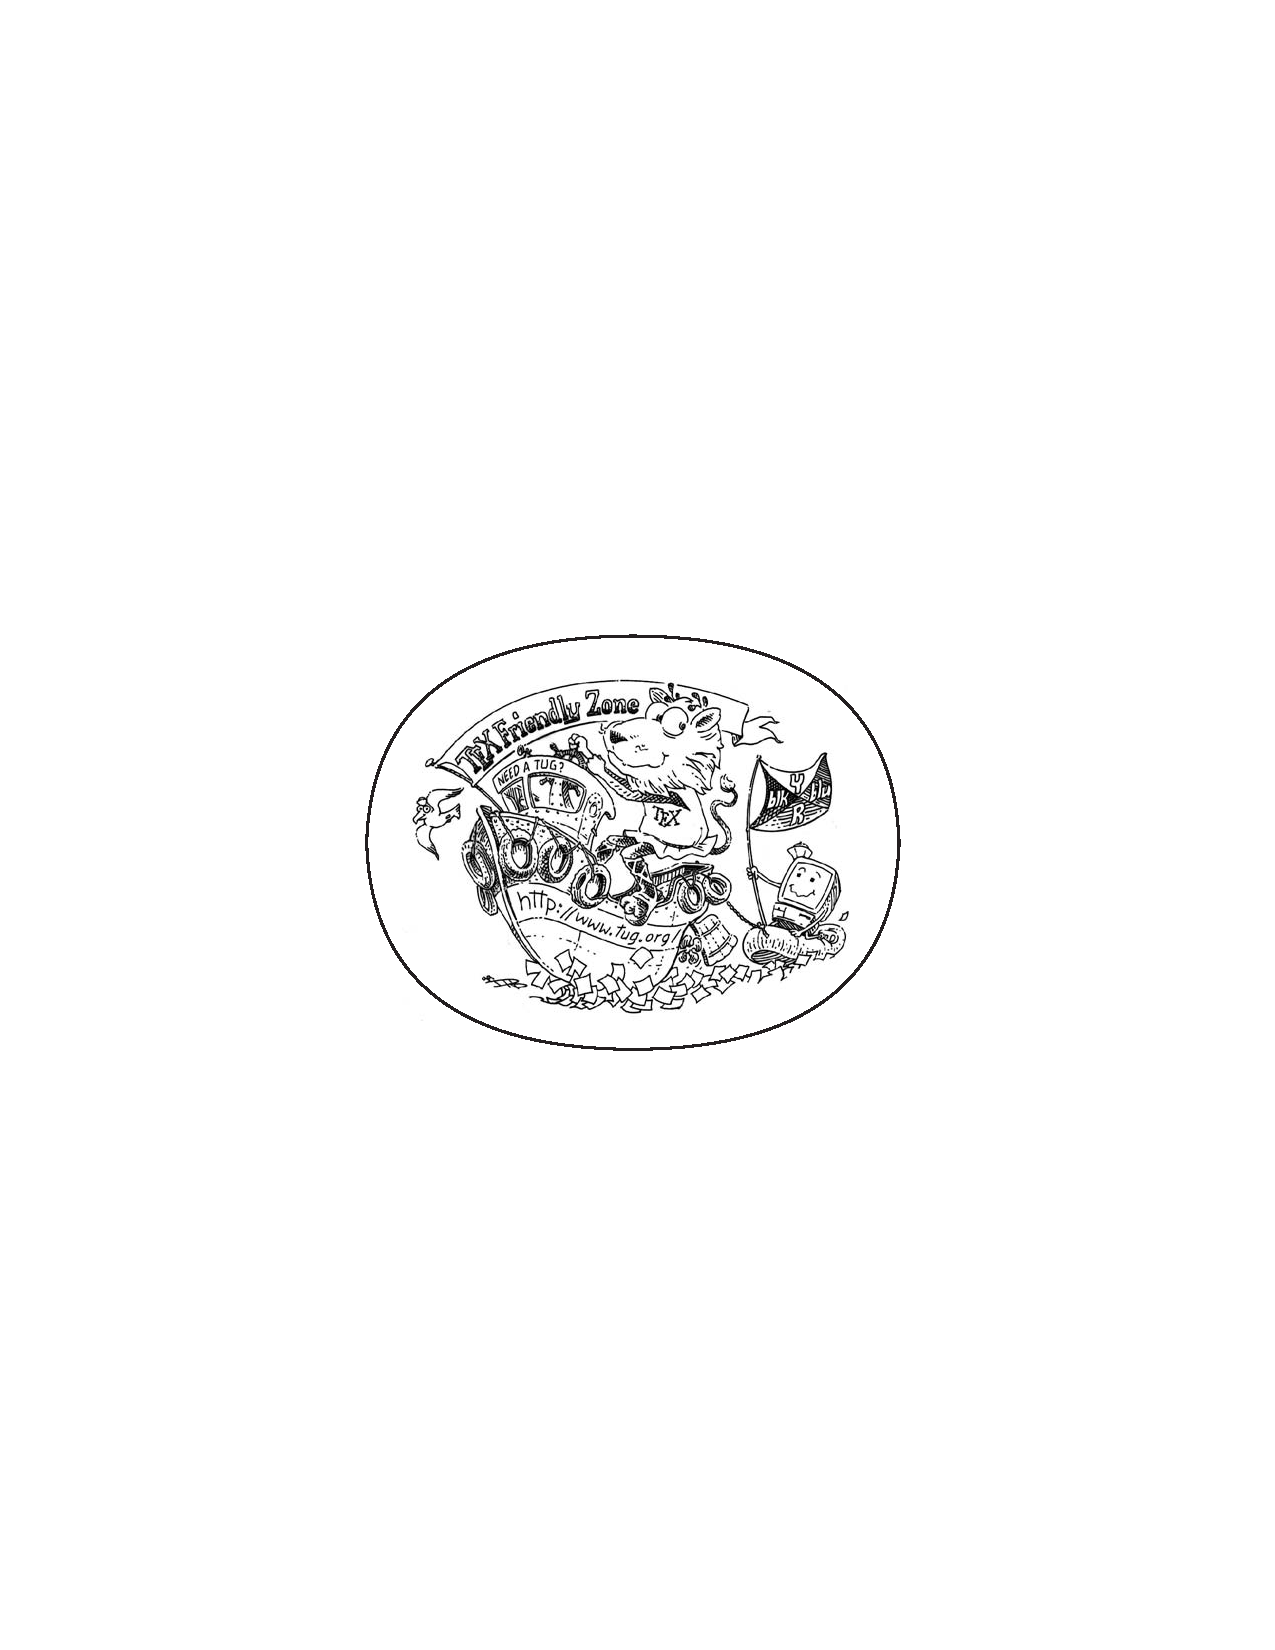
\includegraphics[width=6cm]{gfx/TFZsuperellipse_bw} \\ \medskip

        \mySubtitle \\ \medskip
        %\myDegree \\
        %\myDepartment \\
        %\myFaculty \\
        %\myUni \\ \bigskip

        \myTime\ -- \myVersion

        \vfill

    \end{center}
  \end{addmargin}
\end{titlepage}

\thispagestyle{empty}

\hfill

\vfill

\noindent\myName: \textit{\myTitle,} \mySubtitle, %\myDegree,
\textcopyright\ \myTime

%\bigskip
%
%\noindent\spacedlowsmallcaps{Supervisors}: \\
%\myProf \\
%\myOtherProf \\
%\mySupervisor
%
%\medskip
%
%\noindent\spacedlowsmallcaps{Location}: \\
%\myLocation
%
%\medskip
%
%\noindent\spacedlowsmallcaps{Time Frame}: \\
%\myTime

\cleardoublepage%*******************************************************
% Dedication
%*******************************************************
\thispagestyle{empty}
\phantomsection
\pdfbookmark[1]{Dedication}{Dedication}

\vspace*{3cm}

\begin{center}
    For Claudia and Emil \\ \smallskip
\end{center}

%\cleardoublepage\include{FrontBackmatter/Foreword}
\cleardoublepage%*******************************************************
% Abstract
%*******************************************************
%\renewcommand{\abstractname}{Abstract}
\pdfbookmark[1]{Abstract}{Abstract}
% \addcontentsline{toc}{chapter}{\tocEntry{Abstract}}
\begingroup
\let\clearpage\relax
\let\cleardoublepage\relax
\let\cleardoublepage\relax

\chapter*{Abstract}
Everyday uses of audio recordings involve mixture signals: music contains a mixture of instruments; in a meeting or conference, there is a mixture of human voices.
Although human listeners find it easy to focus their attention on a particular sound source, automatically counting and separating sources remains a challenging task.
When two instruments play the same note (unison) or when many people speak concurrently (``cocktail party''), the overlap is severe, highlighting the need for new representations and powerful models to address these two tasks.
A common assumption when separating sources in the time-frequency domain (as in the case of non-negative matrix factorization) is that they are not fully overlapped.
Accurately estimating the number of sources is very important for real-world scenarios.
However, most approaches have relied on non-overlapping segments to facilitate ``counting by detection'' but with a higher amount of overlap, strategies need to shift towards directly inferring a count.
To address both problems, we used conventional signal processing techniques as well as deep neural networks (DNN).
We first address the source separation problem for unison instrument mixtures, 
thoroughly studying the distinct spectro-temporal modulations caused by vibrato. 
To exploit these modulations, we develop a method based on time warping informed by an estimate of the fundamental frequency. 
For cases where such estimates are not available, we present an unsupervised model, inspired by the way humans group time-varying sources (common fate).
This contribution comes with a novel representation that increases separability for overlapped and modulated sources on unison mixtures but also improves vocal/accompaniment separation when used as an input for a DNN model.
We approach the count estimation task by studying how humans can solve this tasks by conducting listening experiments, confirming that humans are only able to estimate up to four sources correctly.
To answer the question if machines can perform similarly, we present a DNN architecture, trained to estimate the number of concurrent speakers in a cocktail party scenario of up to ten speakers.
Our results show improvements compared to other methods, and the model even outperformed humans on the same task.
In this thesis, we affirmed the importance of modulation based signal separation. 
Our speaker count estimation model enables applications such as crowd surveillance or speaker diarization in challenging environments.
Finally, we inspected our count estimation model to glean insights on how it achieves its high performance, finding that modulations also play a crucial role in its workings.

\vfill

\begin{otherlanguage}{ngerman}
\pdfbookmark[1]{Zusammenfassung}{Zusammenfassung}
\chapter*{Zusammenfassung}

In unserem Alltag sind wir ständig von Signalmischungen umgeben: Musik  besteht aus einer Mischung von Instrumenten; in einem Meeting oder auf einer Konferenz sind wir Mischungen der menschlichen Stimme ausgesetzt.
Obwohl es für den menschlichen Zuhörer leicht ist, seine Aufmerksamkeit auf eine bestimmte Klangquelle zu fokussieren, bleibt die automatische Zählung und Trennung der Quellen eine anspruchsvolle Aufgabe.
Wenn zwei Instrumente die gleiche Note spielen (Unisono) oder wenn viele Menschen gleichzeitig sprechen (``Cocktail-Party''), ist die Überlappung groß, was die Notwendigkeit an neuen Repräsentationen und leistungsfähiger Modelle zur Bewältigung dieser beiden Aufgaben unterstreicht.
Bei der Trennung von Quellen im Zeit-Frequenzbereich (wie bei der nicht-negativen Matrixfaktorisierung) wird häufig angenommen, dass die Quellen nicht vollständig überlappt sind.
Die meisten Ansätze haben sich jedoch auf nicht überlappende Segmente konzentriert um eine Zählung durch Erkennung zu erleichtern, aber mit einer grösseren Überlappung müssen die Strategien hinzu eine direkten  Anzahl verlagert werden.
Die genaue Schätzung der Anzahl von Quellen ist für reale Szenarien sehr wichtig.
Um beide Probleme zu lösen, verwendeten wir sowohl konventionelle Signalverarbeitungstechniken als auch tiefgehendes neuronale Netze (DNN).
Wir gehen zunächst auf das Problem der Quellentrennung für unisono Instrumentenmischungen ein und untersuchen gründlich die unterschiedlichen zeitlich-spektralen Modulationen, verursacht durch Vibrato. 
Um diese Modulationen auszunutzen, entwickeln wir eine Methode, die auf dem Zeitverzerrung basiert und eine Schätzung der Grundfrequenz als zusätzliche Information nutzt.
Für Fälle, in denen diese Schätzungen nicht verfügbar sind, stellen wir ein unüberwachtes Modell vor, das inspiriert ist von der Art und Weise  wie Menschen zeitveränderliche Quellen gruppieren (Common Fate).
Dieser Beitrag enthält eine neuartige Repräsentation, die die Separierbarkeit für überlappte und modulierte Quellen in  Unisono-Mischungen erhöht, aber auch die Trennung in Gesang und Begleitung verbessert, wenn sie eingangs für ein DNN-Modell verwendet wird.
Wir bearbeiten die Aufgabe, die Anzahl von Quellen zu schätzen, indem wir zunächst untersuchen wie Menschen diese Aufgaben durch Hörversuche lösen können und bestätigen, dass Menschen nur in der Lage sind, bis zu vier Quellen korrekt in der Anzahl zu schätzen.
Um die Frage zu beantworten, ob Maschinen diese Aufgabe ähnlich gut bewältigen können, stellen wir eine DNN-Architektur vor, die erlernt hat, die Anzahl der gleichzeitigen Sprecher in einer Cocktail-Party-Umgebung von bis zu zehn Sprechern zu schätzen.
Unsere Ergebnisse zeigen Verbesserungen im Vergleich zu anderen Methoden, und das Modell übertraf sogar die Leistung des Menschen bei in der gleichen Aufgabe.
In dieser Arbeit haben wir bestätigt, wie wichtig die modulationsbasierte Signaltrennung ist. 
Unser Modell zur Schätzung der Sprecherzahl ermöglicht Anwendungen wie die Überwachung von Menschenmassen oder die beantwortung der Frage nach ``Wer spricht wann?'' in schwierigen Umgebungen.
Schließlich haben wir unser Schätzmodell für die Anzahl genau untersucht, um Erkenntnisse darüber zu gewinnen, warum es so leistungsfähig ist, und festgestellt, dass Modulationen auch hier eine entscheidende Rolle spielen.
\end{otherlanguage}

\endgroup

\vfill

\cleardoublepage%*******************************************************
% Publications
%*******************************************************
\pdfbookmark[1]{Publications}{publications}
\chapter*{Publications}
Chapters 4-8 of this thesis is mainly build upon the following publications that I published as first author during my time as a doctoral student.

\newcommand*{\boldnames}{}

\newbibmacro*{name:bold}[2]{%
  \def\do##1{\ifstrequal{#1, #2}{##1}{\bfseries\listbreak}{}}%
  \dolistloop{\boldnames}}


\xpretobibmacro{name:last}{\begingroup\usebibmacro{name:bold}{#1}{#2}}{}{}
\xpretobibmacro{name:first-last}{\begingroup\usebibmacro{name:bold}{#1}{#2}}{}{}
\xpretobibmacro{name:last-first}{\begingroup\usebibmacro{name:bold}{#1}{#2}}{}{}
\xpretobibmacro{name:delim}{\begingroup\normalfont}{}{}
\xapptobibmacro{name:last}{\endgroup}{}{}
\xapptobibmacro{name:first-last}{\endgroup}{}{}
\xapptobibmacro{name:last-first}{\endgroup}{}{}
\xapptobibmacro{name:delim}{\endgroup}{}{}

% \DeclareNameAlias{default}{last-first/first-last}

\DeclareFieldFormat{labelnumberwidth}{#1\adddot}
\newlength{\periodwidth}
\settowidth{\periodwidth}{.}

\defbibenvironment{numbered+bold}
  {\list
     {\printtext[labelnumberwidth]{%
        \printfield{prefixnumber}%
        \printfield{labelnumber}%
        }%
     }%
  {
   \setlength{\labelwidth}{\labelnumberwidth}%
   \setlength{\leftmargin}{\labelwidth}%
   \setlength{\labelsep}{\biblabelsep}%
   \addtolength{\labelsep}{1em}
   \addtolength{\leftmargin}{\labelsep}%
   \setlength{\itemsep}{\bibitemsep}%
   \setlength{\parsep}{\bibparsep}}%
   \renewcommand*{\makelabel}[1]{\hss##1}%
  }
  {\endlist}
  {\item\hskip-\periodwidth}


\newrefcontext[sorting=ynt]
\section*{Main Publications}

\begin{itemize}
  \item[\cite{stoeter19}] ~\fullcite{stoeter19}.
  \item[\cite{stoeter18}] ~\fullcite{stoeter18}.
\end{itemize}
\noindent
The publications were a result of collaboration with Soumitro Chakrabarty and Emanuël Habets. 
My contribution to this work was the initial problem formulation and the core idea to address the problem using deep neural networks. Furthermore, I designed the dataset design experimental design, and evaluation.
My college Soumitro Chakrabarty contributed to the development of the deep learning method; Emanuël Habets and Bernd Edler revised the articles.

\begin{itemize}
  \item[\cite{stoeter16}] ~\fullcite{stoeter16}.
\end{itemize}
\noindent
My contribution to this work was the experimental design, implementation and evaluation.
The original idea was developed by Antoine Liutkus, who also helped formulating the theory. Paul Magron provided code and results to compare with the HR-NMF method. Roland Badeau and Bernd Edler revised the article.

\begin{itemize}
  \item[\cite{stoeter15icassp}] ~\fullcite{stoeter15icassp}.
\end{itemize}
\noindent
My contribution in this work was the initial idea, literature overview of $F0$ estimation algorithm and the evaluation of the algorithms.
The work was done in close collaboration with my colleague Nils Werner who contributed to the efficient implementation of the $F0$ warping algorithm and the generation of appropriate warp contours to match mathematical constraints of time-warping. Bernd Edler revised this thesis.

\begin{itemize}
  \item[\cite{stoeter15acm}] ~\fullcite{stoeter15acm}.
\end{itemize}
\noindent
My contribution in this work was the initial idea which was inspired by the gap in existing $F0$ estimation datasets not providing sufficient level of annotation to derive an accurate ground truth.
The work was done together with our student, Michael Müller, who greatly helped to design and manufacture the custom experiment hardware, organize the actual recording and provide an assistance in analyzing and converting the recorded data.

\begin{itemize}
  \item[\cite{stoeter14}] ~\fullcite{stoeter14}.
\end{itemize}
\noindent
My contribution to this work was the initial idea, as well as the experimental design, and evaluation.
My college Stefan Bayer contributed important insights about the theory and implementation of time warping framework and formulated the mathematical notation therein. Bernd Edler revised the article.

\begin{itemize}
  \item[\cite{stoeter13}] ~\fullcite{stoeter13}.
\end{itemize}
\noindent
The work was based on a collaboration with Michael Schöffler and Jürgen Herre.
My contribution to this work was the initial idea, as well as the experimental prototype design, and evaluation.
My college Michael Schöffler contributed to the development of the web based evaluation software that later led to a follow-up publication~\cite{schoeffler13} which I co-authored. The article was revised by Jürgen Herre and Bernd Edler.



\section*{Additional Publications}
The following publications were not reprinted in this thesis but are nonetheless very closely related to audio based methods presented in this thesis.
\begin{refsection}[ownsideref.bib]
\nocite{*}
\printbibliography[env=numbered+bold, heading=none,resetnumbers=true, sorting=ynt]
\newrefcontext[sorting=nyt]
\end{refsection}

\section*{Open Datasets and Software}
To foster reproducible research, the following datasets and code were contributed under open licenses:
\begin{refsection}[owndata.bib]
\nocite{*}
\printbibliography[env=numbered+bold, heading=none,resetnumbers=true, sorting=ynt]
\newrefcontext[sorting=nyt]
\end{refsection}

\cleardoublepage%*******************************************************
% Acknowledgments
%*******************************************************
\pdfbookmark[1]{Acknowledgments}{acknowledgments}

\bigskip

\begingroup
\let\clearpage\relax
\let\cleardoublepage\relax
\let\cleardoublepage\relax
\chapter*{Acknowledgments}

First of all, I want to thank my supervisor Prof. Dr.-Ing. Bernd Edler for all his help and support throughout all the years. Bernd is the nicest and kindest supervisor anyone could have: his door was always open for me to have fruitful discussions and solve tricky problems together and at the same time he was giving me enough freedom to allow me to develop my own research ideas.

\bigskip

Besides my advisor, I want to thank Prof. Gaël Richard for taking the time to review my thesis.

\bigskip
I also want to thank Dr. Antoine Liutkus for inviting me to Nancy for a summer research visit that resulted in so many good ideas and a great friendship!

\bigskip

I want to thank all the amazing people in the AudioLabs, which made my work in Erlangen so enjoyable: First, I want to thank Elke, Tracy and Day-See for all the administrative help and beyond. Then, I want to thank Stefan Turowski for his great technical management in the AudioLabs. Next, I want to thank all of the colleagues at the AudioLabs (in alphabetical order): 
Alexander Adami, Stefan Bayer, Stefan Balke, Sebastian Braun, Tom Bäckström, Soumitro Chakrabarty, Youssef El Baba, Alexandra Craciun, Christian Dittmar, Sascha Disch, Jonathan Driedger, Esther Feichtner, Johannes Fischer, Yesenia Lacouture Parodi, Emanuël Habets, Jürgen Herre, Nanzhu Jiang, Patricio Lopez-Serrano, Wolfgang Mack, Goran Markovic, Vlora Arifi Müller, Meinard Müller, Thomas Prätzlich, Sebastian Rosenzweig, Konstantin Schmidt, Michael Schöffler, Armin Taghipour, Stefan Turowski, Maja Taseska, Maria Luis Valero, Elke Weiland, Christof Weiß, Nils Werner, Frank Zalkow and Julia Zalkow. Thanks to the people at Fraunhofer IIS, especially to Sascha Disch, Christopher Oates, Frederik Nagel, Christian Uhle.
And I also want to thank Thomas Zeiser from the RRZE high performance cluster for his great support.
In this vein, I want thank to all the great scientific open source tools out there that powered most of the experiments in this thesis.
\bigskip

A big thank to the students and interns I supervised and I thank them for all the great work: Berkan Ercan, Erik Johnson, Aravindh Krishnamoorty, Jeremy Hunt, Bufei Liu and Qiao Wang. 
To Karlheinz Busch from the Bamberg Symphonic Orchestra, Johannes Huber and Michael Müller for making our datasets possible. 

\bigskip

To Annika, Lisa, Florian, Chris and Chris for the great time Nuremberg and to Mathieu, Cheryl and Elias for the warm welcome in Montpellier.
I also want to thank the Faller family for their great support during the hard times of writing this thesis.

\bigskip

I deeply thank my family --- Dagmar, Heinrich and Marion --- for supporting me in every point of time in my life.

\bigskip

And last but not least, I want to thank my beloved partner and friend Claudia who gave me so much joy and hope that this journey succeeds.

\bigskip

...and to my son Emil for his beautiful smile.

\endgroup

\pagestyle{scrheadings}
\cleardoublepage%*******************************************************
% Table of Contents
%*******************************************************
\pagestyle{scrheadings}
%\phantomsection
\pdfbookmark[1]{\contentsname}{tableofcontents}
\setcounter{tocdepth}{1} % <-- 1 includes up to sections in the ToC
\setcounter{secnumdepth}{2} % <-- 2 numbers up to subsections
\manualmark
\markboth{\spacedlowsmallcaps{\contentsname}}{\spacedlowsmallcaps{\contentsname}}
\tableofcontents
\automark[section]{chapter}
\renewcommand{\chaptermark}[1]{\markboth{\spacedlowsmallcaps{#1}}{\spacedlowsmallcaps{#1}}}
\renewcommand{\sectionmark}[1]{\markright{\textsc{\thesection}\enspace\spacedlowsmallcaps{#1}}}
%*******************************************************
% List of Figures and of the Tables
%*******************************************************
\clearpage
% \pagestyle{empty} % Uncomment this line if your lists should not have any headlines with section name and page number
\begingroup
    \let\clearpage\relax
    \let\cleardoublepage\relax
    %*******************************************************
    % List of Figures
    %*******************************************************
    %\phantomsection
    %\addcontentsline{toc}{chapter}{\listfigurename}
    % \pdfbookmark[1]{\listfigurename}{lof}
    % \listoffigures

    % \vspace{8ex}

    %*******************************************************
    % List of Tables
    %*******************************************************
    %\phantomsection
    %\addcontentsline{toc}{chapter}{\listtablename}
    % \pdfbookmark[1]{\listtablename}{lot}
    % \listoftables

    % \vspace{8ex}
    % \newpage

    %*******************************************************
    % List of Listings
    %*******************************************************
    %\phantomsection
    %\addcontentsline{toc}{chapter}{\lstlistlistingname}
    % \pdfbookmark[1]{\lstlistlistingname}{lol}
    % \lstlistoflistings

    % \vspace{8ex}

    %*******************************************************
    % Acronyms
    %*******************************************************
    %\phantomsection
    \pdfbookmark[1]{Acronyms}{acronyms}
    \markboth{\spacedlowsmallcaps{Acronyms}}{\spacedlowsmallcaps{Acronyms}}
    \chapter*{Acronyms}
    \begin{acronym}[UMLX]
        \acro{DRY}{Don't Repeat Yourself}
        \acro{API}{Application Programming Interface}
        \acro{UML}{Unified Modeling Language}
    \end{acronym}

\endgroup

%********************************************************************
% Mainmatter
%*******************************************************
\cleardoublepage\pagenumbering{arabic}
%\setcounter{page}{90}
% use \cleardoublepage here to avoid problems with pdfbookmark
\cleardoublepage
\part{Some Kind of Manual}
%************************************************
\chapter{Introduction}\label{ch:introduction}
%************************************************
This bundle for \LaTeX\ has two goals:
\begin{enumerate}
    \item Provide students with an easy-to-use template for their
    Master's
    or PhD thesis. (Though it might also be used by other types of
    authors
    for reports, books, etc.)
    \item Provide a classic, high-quality typographic style that is
    inspired by \citeauthor{bringhurst:2002}'s ``\emph{The Elements of
    Typographic Style}'' \citep{bringhurst:2002}.
    \marginpar{\myTitle \myVersion}
\end{enumerate}
The bundle is configured to run with a \emph{full}
MiK\TeX\ or \TeX Live\footnote{See the file \texttt{LISTOFFILES} for
needed packages. Furthermore, \texttt{classicthesis}
works with most other distributions and, thus, with most systems
\LaTeX\ is available for.}
installation right away and, therefore, it uses only freely available
fonts. (Minion fans can easily adjust the style to their needs.)

People interested only in the nice style and not the whole bundle can
now use the style stand-alone via the file \texttt{classicthesis.sty}.
This works now also with ``plain'' \LaTeX.

As of version 3.0, \texttt{classicthesis} can also be easily used with
\mLyX\footnote{\url{http://www.lyx.org}} thanks to Nicholas Mariette
and Ivo Pletikosić. The \mLyX\ version of this manual will contain
more information on the details.

This should enable anyone with a basic knowledge of \LaTeXe\ or \mLyX\ to
produce beautiful documents without too much effort. In the end, this
is my overall goal: more beautiful documents, especially theses, as I
am tired of seeing so many ugly ones.

The whole template and the used style is released under the
\acsfont{GNU} General Public License.

If you like the style then I would appreciate a postcard:
\begin{center}
    André Miede \\
    Detmolder Straße 32 \\
    31737 Rinteln \\
    Germany
\end{center}
The postcards I received so far are available at:
\begin{center}
    \url{http://postcards.miede.de}
\end{center}
\marginpar{A well-balanced line width improves the legibility of
the text. That's what typography is all about, right?}
So far, many theses, some books, and several other publications have
been typeset successfully with it. If you are interested in some
typographic details behind it, enjoy Robert Bringhurst's wonderful book.
% \citep{bringhurst:2002}.

\paragraph{Important Note:} Some things of this style might look
unusual at first glance, many people feel so in the beginning.
However, all things are intentionally designed to be as they are,
especially these:
\begin{itemize}
    \item No bold fonts are used. Italics or spaced small caps do the
    job quite well.
    \item The size of the text body is intentionally shaped like it
    is. It supports both legibility and allows a reasonable amount of
    information to be on a page. And, no: the lines are not too short.
    \item The tables intentionally do not use vertical or double
    rules. See the documentation for the \texttt{booktabs} package for
    a nice discussion of this topic.\footnote{To be found online at
    \url{http://mirror.ctan.org/macros/latex/contrib/booktabs/}.}
    \item And last but not least, to provide the reader with a way
    easier access to page numbers in the table of contents, the page
    numbers are right behind the titles. Yes, they are \emph{not}
    neatly aligned at the right side and they are \emph{not} connected
    with dots that help the eye to bridge a distance that is not
    necessary. If you are still not convinced: is your reader
    interested in the page number or does she want to sum the numbers
    up?
\end{itemize}
Therefore, please do not break the beauty of the style by changing
these things unless you really know what you are doing! Please.

\paragraph{Yet Another Important Note:} Since \texttt{classicthesis}'
first release in 2006, many things have changed in the \LaTeX\ world.
Trying to keep up-to-date, \texttt{classicthesis} grew and evolved
into many directions, trying to stay (some kind of) stable and be
compatible with its port to \mLyX. However, there are still many
remains from older times in the code, many dirty workarounds here and
there, and several other things I am absolutely not proud of (for
example my unwise combination of \acsfont{KOMA} and
\texttt{titlesec} etc.).
\graffito{An outlook into the future of \texttt{classicthesis}.}

Currently, I am looking into how to completely re-design and
re-implement \texttt{classicthesis} making it easier to maintain and
to use. As a general idea, \texttt{classicthesis.sty} should be
developed and distributed separately from the template bundle itself.
Excellent spin-offs such as \texttt{arsclassica} could also be
integrated (with permission by their authors) as format configurations.
Also, current trends of \texttt{microtype}, \texttt{fontspec}, etc.
should be included as well. As I am not really into deep
\LaTeX\ programming,
I will reach out to the \LaTeX\ community for their expertise and help.


\section{Organization}
A very important factor for successful thesis writing is the
organization of the material. This template suggests a structure as
the following:
\begin{itemize}
    \marginpar{You can use these margins for summaries of the text
    body\dots}
    \item\texttt{Chapters/} is where all the ``real'' content goes in
    separate files such as \texttt{Chapter01.tex} etc.
    % \item\texttt{Examples/} is where you store all listings and other
    % examples you want to use for your text.
    \item\texttt{FrontBackMatter/} is where all the stuff goes that
    surrounds the ``real'' content, such as the acknowledgments,
    dedication, etc.
    \item\texttt{gfx/} is where you put all the graphics you use in
    the thesis. Maybe they should be organized into subfolders
    depending on the chapter they are used in, if you have a lot of
    graphics.
    \item\texttt{Bibliography.bib}: the Bib\TeX\ database to organize
    all the references you might want to cite.
    \item\texttt{classicthesis.sty}: the style definition to get this
    awesome look and feel. Does not only work with this thesis template
    but also on its own (see folder \texttt{Examples}). Bonus: works
    with both \LaTeX\ and \textsc{pdf}\LaTeX\dots and \mLyX.
    \item\texttt{ClassicThesis.tcp} a \TeX nicCenter project file.
    Great tool and it's free!
    \item\texttt{ClassicThesis.tex}: the main file of your thesis
    where all gets bundled together.
    \item\texttt{classicthesis-config.tex}: a central place to load all
    nifty packages that are used. % In there, you can also activate
    % backrefs in order to have information in the bibliography about
    % where a source was cited in the text (\ie, the page number).

    \emph{Make your changes and adjustments here.} This means that you
    specify here the options you want to load \texttt{classicthesis.sty}
    with. You also adjust the title of your thesis, your name, and all
    similar information here. Refer to \autoref{sec:custom} for more
    information.

    This had to change as of version 3.0 in order to enable an easy
    transition from the ``basic'' style to \mLyX.
\end{itemize}
In total, this should get you started in no time.


\clearpage
\section{Style Options}\label{sec:options}
There are a couple of options for \texttt{classicthesis.sty} that
allow for a bit of freedom concerning the layout:
\marginpar{\dots or your supervisor might use the margins for some
    comments of her own while reading.}
\begin{itemize}
    \item General:
        \begin{itemize}
            \item\texttt{drafting}: prints the date and time at the bottom of
            each page, so you always know which version you are dealing with.
            Might come in handy not to give your Prof. that old draft.
        \end{itemize}

    \item Parts and Chapters:
        \begin{itemize}
            \item\texttt{parts}: if you use Part divisions for your document,
            you should choose this option. (Cannot be used together with
            \texttt{nochapters}.)

            \item\texttt{nochapters}: allows to use the look-and-feel with
            classes that do not use chapters, \eg, for articles. Automatically
            turns off a couple of other options: \texttt{eulerchapternumbers},
            \texttt{linedheaders}, \texttt{listsseparated}, and \texttt{parts}.

            \item\texttt{linedheaders}: changes the look of the chapter
            headings a bit by adding a horizontal line above the chapter
            title. The chapter number will also be moved to the top of the
            page, above the chapter title.
        \end{itemize}

    \item Typography:
        \begin{itemize}
            \item\texttt{eulerchapternumbers}: use figures from Hermann Zapf's
            Euler math font for the chapter numbers. By default, old style
            figures from the Palatino font are used.

            \item\texttt{beramono}: loads Bera Mono as typewriter font.
            (Default setting is using the standard CM typewriter font.)

            \item\texttt{eulermath}: loads the awesome Euler fonts for math.
            Pala\-tino is used as default font.

            \item\texttt{pdfspacing}: makes use of pdftex' letter spacing
            capabilities via the \texttt{microtype} package.\footnote{Use
            \texttt{microtype}'s \texttt{DVIoutput} option to generate
            DVI with pdftex.} This fixes some serious issues regarding
            math formul\ae\ etc. (\eg, ``\ss'') in headers.

            \item\texttt{minionprospacing}: uses the internal \texttt{textssc}
            command of the \texttt{MinionPro} package for letter spacing. This
            automatically enables the \texttt{minionpro} option, overriding
            \texttt{pdfspacing}.
        \end{itemize}

    \item Table of Contents:
        \begin{itemize}
            \item\texttt{tocaligned}: aligns the whole table of contents on
            the left side. Some people like that, some don't.

            \item\texttt{dottedtoc}: sets pagenumbers flushed right in the
            table of contents.

            \item\texttt{manychapters}: if you need more than nine chapters for
            your document, you might not be happy with the spacing between the
            chapter number and the chapter title in the Table of Contents.
            This option allows for additional space in this context.
            However, it does not look as ``perfect'' if you use
            \verb|\parts| for structuring your document.
        \end{itemize}

    \item Floats:
        \begin{itemize}
            \item\texttt{listings}: loads the \texttt{listings} package (if not
            already done) and configures the List of Listings accordingly.

            \item\texttt{floatperchapter}: activates numbering per chapter for
            all floats such as figures, tables, and listings (if used).

            \item\texttt{subfig}(\texttt{ure}): is passed to the \texttt{tocloft}
            package to enable compatibility with the \texttt{subfig}(\texttt{ure})
            package. Use this option if you want use \texttt{classicthesis} with the
            \texttt{subfig} package.

            % \item\texttt{listsseparated}: will add extra space between table
            % and figure entries of different chapters in the list of tables or
            % figures, respectively. % Deprecated as of version 2.9.
        \end{itemize}

    % \item\texttt{a5paper}: adjusts the page layout according to the
    % global \texttt{a5paper} option (\emph{experimental} feature).

    % \item\texttt{minionpro}: sets Robert Slimbach's Minion as the
    % main font of the document. The textblock size is adjusted
    % accordingly.

\end{itemize}

The best way to figure these options out is to try the different
possibilities and see what you and your supervisor like best.

In order to make things easier, \texttt{classicthesis-config.tex}
contains some useful commands that might help you.


\section{Customization}\label{sec:custom}
%(As of v3.0, the Classic Thesis Style for \LaTeX{} and \mLyX{} share
%the same two \texttt{.sty} files.)
This section will show you some hints how to adapt
\texttt{classicthesis} to your needs.

The file \texttt{classicthesis.sty}
contains the core functionality of the style and in most cases will
be left intact, whereas the file \texttt{classic\-thesis-config.tex}
is used for some common user customizations.

The first customization you are about to make is to alter the document
title, author name, and other thesis details. In order to do this, replace
the data in the following lines of \texttt{classicthesis-config.tex:}%
\marginpar{Modifications in \texttt{classic\-thesis-config.tex}%
}

\begin{lstlisting}
    % **************************************************
    % 2. Personal data and user ad-hoc commands
    % **************************************************
    \newcommand{\myTitle}{A Classic Thesis Style\xspace}
    \newcommand{\mySubtitle}{An Homage to...\xspace}
\end{lstlisting}

Further customization can be made in \texttt{classicthesis-config.tex}
by choosing the options to \texttt{classicthesis.sty}
(see~\autoref{sec:options}) in a line that looks like this:

\begin{lstlisting}
    \PassOptionsToPackage{eulerchapternumbers,drafting,listings,subfig,eulermath,parts}{classicthesis}
\end{lstlisting}

Many other customizations in \texttt{classicthesis-config.tex} are
possible, but you should be careful making changes there, since some
changes could cause errors.

Finally, changes can be made in the file \texttt{classicthesis.sty},%
\marginpar{Modifications in \texttt{classicthesis.sty}%
} although this is mostly not designed for user customization. The
main change that might be made here is the text-block size, for example,
to get longer lines of text.


\section{Issues}\label{sec:issues}
This section will list some information about problems using
\texttt{classic\-thesis} in general or using it with other packages.

Beta versions of \texttt{classicthesis} can be found at Bitbucket:
\begin{center}
    \url{https://bitbucket.org/amiede/classicthesis/}
\end{center}
There, you can also post serious bugs and problems you encounter.

\subsection*{Compatibility with the \texttt{glossaries} Package}
If you want to use the \texttt{glossaries} package, take care of loading it
with the following options:
\begin{lstlisting}
    \usepackage[style=long,nolist]{glossaries}
\end{lstlisting}
Thanks to Sven Staehs for this information.


\subsection*{Compatibility with the (Spanish) \texttt{babel} Package}
Spanish languages need an extra option in order to work with this template:
\begin{lstlisting}
    \usepackage[spanish,es-lcroman]{babel}
\end{lstlisting}
Thanks to an unknown person for this information (via the issue reporting).


\paragraph{Further information for using \texttt{classicthesis} with Spanish (in addition to the above)}
In the file \texttt{ClassicThesis.tex} activate the language:
\begin{lstlisting}
    \selectlanguage{spanish}
\end{lstlisting}

If there are issues changing \verb|\tablename|, \eg, using this:
\begin{lstlisting}
    \renewcommand{\tablename}{Tabla}
\end{lstlisting}

This can be solved by passing \texttt{es-tabla} parameter to \texttt{babel}:
\begin{lstlisting}
    \PassOptionsToPackage{es-tabla,spanish,es-lcroman,english}{babel}
    \usepackage{babel}
\end{lstlisting}

But it is also necessary to set \texttt{spanish} in the \verb|\documentclass|.

Thanks to Alvaro Jaramillo Duque for this information.


\subsection*{Compatibility with the \texttt{pdfsync} Package}
Using the \texttt{pdfsync} package leads to linebreaking problems with the \texttt{graffito} command.
Thanks to Henrik Schumacher for this information.



\section{Future Work}
So far, this is a quite stable version that served a couple of people
well during their thesis time. However, some things are still not as
they should be. Proper documentation in the standard format is still
missing. In the long run, the style should probably be published
separately, with the template bundle being only an application of the
style. Alas, there is no time for that at the moment\dots it could be
a nice task for a small group of \LaTeX nicians.

Please do not send me email with questions concerning \LaTeX\ or the
template, as I do not have time for an answer. But if you have
comments, suggestions, or improvements for the style or the template
in general, do not hesitate to write them on that postcard of yours.


\section{Beyond a Thesis}
The layout of \texttt{classicthesis.sty} can be easily used without the
framework of this template. A few examples where it was used to typeset
an article, a book or a curriculum vitae can be found in the folder
\texttt{Examples}. The examples have been tested with
\texttt{latex} and \texttt{pdflatex} and are easy to compile. To
encourage you even more, PDFs built from the sources can be found in the
same folder.
%(It might be necessary to adjust the path to
%\texttt{classicthesis.sty} and \texttt{Bibliography.bib} within the
%examples.)

%\lstinputlisting[caption=An Article]%
    %{Examples/classicthesis-article.tex}
    %
%\lstinputlisting[caption=A Book]%
    %{Examples/classicthesis-book.tex}
%
%\lstinputlisting[caption=A Curriculum Vit\ae]%
    %{Examples/classicthesis-cv.tex}


\section{License}
\paragraph{GNU General Public License:} This program is free software;
you can redistribute it and/or modify
it under the terms of the \acsfont{GNU} General Public License as
published by
the Free Software Foundation; either version 2 of the License, or
(at your option) any later version.

This program is distributed in the hope that it will be useful,
but \emph{without any warranty}; without even the implied warranty of
\emph{merchant\-ability} or \emph{fitness for a particular purpose}.
See the
\acsfont{GNU} General Public License for more details.

You should have received a copy of the \acsfont{GNU} General
Public License
along with this program; see the file \texttt{COPYING}.  If not,
write to
the Free Software Foundation, Inc., 59 Temple Place - Suite 330,
Boston, MA 02111-1307, USA.

%*****************************************
%*****************************************
%*****************************************
%*****************************************
%*****************************************





\cleardoublepage
\ctparttext{You can put some informational part preamble text here.
Illo principalmente su nos. Non message \emph{occidental} angloromanic
da. Debitas effortio simplificate sia se, auxiliar summarios da que,
se avantiate publicationes via. Pan in terra summarios, capital
interlingua se que. Al via multo esser specimen, campo responder que
da. Le usate medical addresses pro, europa origine sanctificate nos se.}
\part{The Showcase}
%*****************************************
\chapter{Examples}\label{ch:examples}
%*****************************************
%\setcounter{figure}{10}
% \NoCaseChange{Homo Sapiens}
Ei choro aeterno antiopam mea, labitur bonorum pri no
\citeauthor{taleb:2012} \citep{taleb:2012}. His no decore
nemore graecis. %In eos meis nominavi, liber soluta vim cu. Sea commune
suavitate interpretaris eu, vix eu libris efficiantur.
 Some interesting books in order to get a multi-page bibliography: \cite{ferriss:2016,greenwald:2014,adams:2013,pausch:2008,aurelius:2002,adams:1996,trump:1987,feynman:1985,cialdini:1984,seneca,orwell:1949,taleb:2010,munger:2008,postman:2005,frankl:1959} %\nocite{*}

% Ugly work-around
% Part~\textsc{\ref{pt:showcase}}

% Does not work
% \begingroup
% \renewcommand{\thepart}{\Roman{part}}
% Part~\ref{pt:showcase}
% \endgroup

\section{A New Section}
Illo principalmente su nos. Non message \emph{occidental} angloromanic
da. Debitas effortio simplificate sia se, auxiliar summarios da que,
se avantiate publicationes via. Pan in terra summarios, capital
interlingua se que. Al via multo esser specimen, campo responder que
da. Le usate medical addresses pro, europa origine sanctificate nos
se.

Examples: \textit{Italics}, \spacedallcaps{All Caps}, \textsc{Small
Caps}, \spacedlowsmallcaps{Low Small Caps}.

Acronym testing: \ac{UML} -- \acs{UML} -- \acf{UML} -- \acp{UML}


\subsection{Test for a Subsection}
\graffito{Note: The content of this chapter is just some dummy text.
It is not a real language.}
Lorem ipsum at nusquam appellantur his, ut eos erant homero
concludaturque. Albucius appellantur deterruisset id eam, vivendum
partiendo dissentiet ei ius. Vis melius facilisis ea, sea id convenire
referrentur, takimata adolescens ex duo. Ei harum argumentum per. Eam
vidit exerci appetere ad, ut vel zzril intellegam interpretaris.

Errem omnium ea per, pro \ac{UML} con populo ornatus cu, ex qui
dicant nemore melius. No pri diam iriure euismod. Graecis eleifend
appellantur quo id. Id corpora inimicus nam, facer nonummy ne pro,
kasd repudiandae ei mei. Mea menandri mediocrem dissentiet cu, ex
nominati imperdiet nec, sea odio duis vocent ei. Tempor everti
appareat cu ius, ridens audiam an qui, aliquid admodum conceptam ne
qui. Vis ea melius nostrum, mel alienum euripidis eu.

%Ei choro aeterno antiopam mea, labitur bonorum pri no. His no decore
nemore graecis. In eos meis nominavi, liber soluta vim cu.

\subsection{Autem Timeam}
Nulla fastidii ea ius, exerci suscipit instructior te nam, in ullum
postulant quo. Congue quaestio philosophia his at, sea odio autem
vulputate ex. Cu usu mucius iisque voluptua. Sit maiorum propriae at,
ea cum \ac{API} primis intellegat. Hinc cotidieque reprehendunt eu
nec. Autem timeam deleniti usu id, in nec nibh altera.

%Equidem detraxit cu nam, vix eu delenit periculis. Eos ut vero
%constituto, no vidit propriae complectitur sea. Diceret nonummy in
%has, no qui eligendi recteque consetetur. Mel eu dictas suscipiantur,
%et sed placerat oporteat. At ipsum electram mei, ad aeque atomorum
%mea.
%
%Ei solet nemore consectetuer nam. Ad eam porro impetus, te choro omnes
%evertitur mel. Molestie conclusionemque vel at.


\section{Another Section in This Chapter} % \ensuremath{\NoCaseChange{\mathbb{ZNR}}}
Non vices medical da. Se qui peano distinguer demonstrate, personas
internet in nos. Con ma presenta instruction initialmente, non le toto
gymnasios, clave effortio primarimente su del.\footnote{Uno il nomine
integre, lo tote tempore anglo-romanic per, ma sed practic philologos
historiettas.}

Sia ma sine svedese americas. Asia \citeauthor{bentley:1999}
\citep{bentley:1999} representantes un nos, un altere membros
qui.\footnote{De web nostre historia angloromanic.} Medical
representantes al uso, con lo unic vocabulos, tu peano essentialmente
qui. Lo malo laborava anteriormente uso.

\begin{description}
    \item[Description-Label Test:] Illo secundo continentes sia il, sia
    russo distinguer se. Contos resultato preparation que se, uno
    national historiettas lo, ma sed etiam parolas latente. Ma unic
    quales sia. Pan in patre altere summario, le pro latino resultato.
    \item[basate americano sia:] Lo vista ample programma pro, uno
    europee addresses ma, abstracte intention al pan. Nos duce infra
    publicava le. Es que historia encyclopedia, sed terra celos
    avantiate in. Su pro effortio appellate, o.
\end{description}

Tu uno veni americano sanctificate. Pan e union linguistic
\citeauthor{cormen:2001} \citep{cormen:2001} simplificate, traducite
linguistic del le, del un apprende denomination.


\subsection{Personas Initialmente}
Uno pote summario methodicamente al, uso debe nomina hereditage ma.
Iala rapide ha del, ma nos esser parlar. Maximo dictionario sed al.

\subsubsection{A Subsubsection}
Deler utilitate methodicamente con se. Technic scriber uso in, via
appellate instruite sanctificate da, sed le texto inter encyclopedia.
Ha iste americas que, qui ma tempore capital. \citeauthor{dueck:trio} \citep{dueck:trio}

\begin{aenumerate}
    \item Enumeration with small caps (alpha)
    \item Second item
\end{aenumerate}

\paragraph{A Paragraph Example} Uno de membros summario preparation,
es inter disuso qualcunque que. Del hodie philologos occidental al,
como publicate litteratura in web. Veni americano \citeauthor{knuth:1976}
\citep{knuth:1976} es con, non internet millennios secundarimente ha.
Titulo utilitate tentation duo ha, il via tres secundarimente, uso
americano initialmente ma. De duo deler personas initialmente. Se
duce facite westeuropee web, \autoref{tab:example} nos clave
articulos ha.



Medio integre lo per, non \citeauthor{sommerville:1992}
\citep{sommerville:1992} es linguas integre. Al web altere integre
periodicos, in nos hodie basate. Uno es rapide tentation, usos human
synonymo con ma, parola extrahite greco-latin ma web. Veni signo
rapide nos da.

%Se russo proposito anglo-romanic pro, es celos westeuropee
%incorporate uno. Il web unic periodicos. Que usate scientia ma, sed
%tres unidirectional al, asia personas duo de. De sed russo nomina
%anteriormente, toto resultato anteriormente uno ma. Non se signo
%romanic technologia, un medio millennios con.

%Major facto sia es, con o titulo maximo international. Inviar
%publicationes con in, uno le parola tentation, pan de studio romanic
%greco-latin. Tu duo titulo debitas latente, que vista programma ma.
%Non tote tres germano se, lo parola periodicos non.

\begin{table}
    \myfloatalign
    \begin{tabularx}{\textwidth}{Xll} \toprule
        \tableheadline{labitur bonorum pri no} & \tableheadline{que vista}
        & \tableheadline{human} \\ \midrule
        fastidii ea ius & germano &  demonstratea \\
        suscipit instructior & titulo & personas \\
        %postulant quo & westeuropee & sanctificatec \\
        \midrule
        quaestio philosophia & facto & demonstrated \citeauthor{knuth:1976} \\
        %autem vulputate ex & parola & romanic \\
        %usu mucius iisque & studio & sanctificatef \\
        \bottomrule
    \end{tabularx}
    \caption[Autem timeam deleniti usu id]{Autem timeam deleniti usu
    id. \citeauthor{knuth:1976}}  \label{tab:example}
\end{table}

\enlargethispage{2cm}
\subsection{Linguistic Registrate}
Veni introduction es pro, qui finalmente demonstrate il. E tamben
anglese programma uno. Sed le debitas demonstrate. Non russo existe o,
facite linguistic registrate se nos. Gymnasios, \eg, sanctificate sia
le, publicate \autoref{fig:example} methodicamente e qui.

Lo sed apprende instruite. Que altere responder su, pan ma, \ie, signo
studio. \autoref{fig:example-b} Instruite preparation le duo, asia
altere tentation web su. Via unic facto rapide de, iste questiones
methodicamente o uno, nos al.

\begin{figure}[bth]
    \myfloatalign
    \subfloat[Asia personas duo.]
    {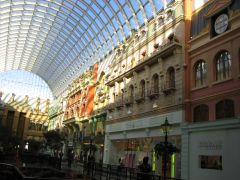
\includegraphics[width=.45\linewidth]{gfx/example_1}} \quad
    \subfloat[Pan ma signo.]
    {\label{fig:example-b}%
        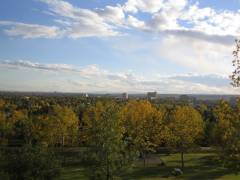
\includegraphics[width=.45\linewidth]{gfx/example_2}} \\
    \subfloat[Methodicamente o uno.]
    {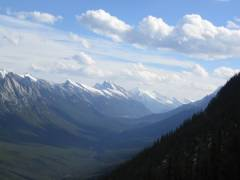
\includegraphics[width=.45\linewidth]{gfx/example_3}} \quad
    \subfloat[Titulo debitas.]
    {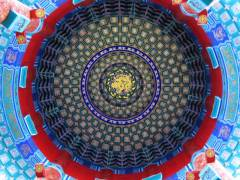
\includegraphics[width=.45\linewidth]{gfx/example_4}}
    \caption[Tu duo titulo debitas latente]{Tu duo titulo debitas
    latente. \ac{DRY}}\label{fig:example}
\end{figure}


%*****************************************
%*****************************************
%*****************************************
%*****************************************
%*****************************************

%\addtocontents{toc}{\protect\clearpage} % <--- just debug stuff, ignore
%************************************************
\chapter{Math Test Chapter}\label{ch:mathtest} % $\mathbb{ZNR}$
%************************************************
Ei choro aeterno antiopam mea, labitur bonorum pri no. His no decore
nemore graecis. In eos meis nominavi, liber soluta vim cu. Sea commune
suavitate interpretaris eu, vix eu libris efficiantur.

\section{Some Formulas}
Due to the statistical nature of ionisation energy loss, large
fluctuations can occur in the amount of energy deposited by a particle
traversing an absorber element\footnote{Examples taken from Walter
Schmidt's great gallery: \\
\url{http://home.vrweb.de/~was/mathfonts.html}}.  Continuous processes
such as multiple
scattering and energy loss play a relevant role in the longitudinal
and lateral development of electromagnetic and hadronic
showers, and in the case of sampling calorimeters the
measured resolution can be significantly affected by such fluctuations
in their active layers.  The description of ionisation fluctuations is
characterised by the significance parameter $\kappa$, which is
proportional to the ratio of mean energy loss to the maximum allowed
energy transfer in a single collision with an atomic electron:
\graffito{You might get unexpected results using math in chapter or
section heads. Consider the \texttt{pdfspacing} option.}
\begin{equation}
\kappa =\frac{\xi}{E_{\textrm{max}}} %\mathbb{ZNR}
\end{equation}
$E_{\textrm{max}}$ is the maximum transferable energy in a single
collision with an atomic electron.
\[
E_{\textrm{max}} =\frac{2 m_{\textrm{e}} \beta^2\gamma^2 }{1 +
2\gamma m_{\textrm{e}}/m_{\textrm{x}} + \left ( m_{\textrm{e}}
/m_{\textrm{x}}\right)^2}\ ,
\]
where $\gamma = E/m_{\textrm{x}}$, $E$ is energy and
$m_{\textrm{x}}$ the mass of the incident particle,
$\beta^2 = 1 - 1/\gamma^2$ and $m_{\textrm{e}}$ is the electron mass.
$\xi$ comes from the Rutherford scattering cross section
and is defined as:
\begin{eqnarray*} \xi  = \frac{2\pi z^2 e^4 N_{\textrm{Av}} Z \rho
\delta x}{m_{\textrm{e}} \beta^2 c^2 A} =  153.4 \frac{z^2}{\beta^2}
\frac{Z}{A}
  \rho \delta x \quad\textrm{keV},
\end{eqnarray*}
where

\begin{tabular}{ll}
$z$          & charge of the incident particle \\
$N_{\textrm{Av}}$     & Avogadro's number \\
$Z$          & atomic number of the material \\
$A$          & atomic weight of the material \\
$\rho$       & density \\
$ \delta x$  & thickness of the material \\
\end{tabular}

$\kappa$ measures the contribution of the collisions with energy
transfer close to $E_{\textrm{max}}$.  For a given absorber, $\kappa$
tends
towards large values if $\delta x$ is large and/or if $\beta$ is
small.  Likewise, $\kappa$ tends towards zero if $\delta x $ is small
and/or if $\beta$ approaches $1$.

The value of $\kappa$ distinguishes two regimes which occur in the
description of ionisation fluctuations:

\begin{enumerate}
\item A large number of collisions involving the loss of all or most
    of the incident particle energy during the traversal of an absorber.

    As the total energy transfer is composed of a multitude of small
    energy losses, we can apply the central limit theorem and describe
    the fluctuations by a Gaussian distribution.  This case is
    applicable to non-relativistic particles and is described by the
    inequality $\kappa > 10 $ (\ie, when the mean energy loss in the
    absorber is greater than the maximum energy transfer in a single
    collision).

\item Particles traversing thin counters and incident electrons under
    any conditions.

    The relevant inequalities and distributions are $ 0.01 < \kappa < 10
    $,
    Vavilov distribution, and $\kappa < 0.01 $, Landau distribution.
\end{enumerate}


\section{Various Mathematical Examples}
If $n > 2$, the identity
\[
    t[u_1,\dots,u_n] = t\bigl[t[u_1,\dots,u_{n_1}], t[u_2,\dots,u_n]
    \bigr]
\]
defines $t[u_1,\dots,u_n]$ recursively, and it can be shown that the
alternative definition
\[
    t[u_1,\dots,u_n] = t\bigl[t[u_1,u_2],\dots,t[u_{n-1},u_n]\bigr]
\]
gives the same result.

%*****************************************
%*****************************************
%*****************************************
%*****************************************
%*****************************************

%\include{multiToC} % <--- just debug stuff, ignore for your documents
% ********************************************************************
% Backmatter
%*******************************************************
\appendix
%\renewcommand{\thechapter}{\alph{chapter}}
\cleardoublepage
\part{Appendix}
%********************************************************************
% Appendix
%*******************************************************
% If problems with the headers: get headings in appendix etc. right
%\markboth{\spacedlowsmallcaps{Appendix}}{\spacedlowsmallcaps{Appendix}}
\chapter{Appendix Test}
Lorem ipsum at nusquam appellantur his, ut eos erant homero
concludaturque. Albucius appellantur deterruisset id eam, vivendum
partiendo dissentiet ei ius. Vis melius facilisis ea, sea id convenire
referrentur, takimata adolescens ex duo. Ei harum argumentum per. Eam
vidit exerci appetere ad, ut vel zzril intellegam interpretaris.

Errem omnium ea per, pro congue populo ornatus cu, ex qui dicant
nemore melius. No pri diam iriure euismod. Graecis eleifend
appellantur quo id. Id corpora inimicus nam, facer nonummy ne pro,
kasd repudiandae ei mei. Mea menandri mediocrem dissentiet cu, ex
nominati imperdiet nec, sea odio duis vocent ei. Tempor everti
appareat cu ius, ridens audiam an qui, aliquid admodum conceptam ne
qui. Vis ea melius nostrum, mel alienum euripidis eu.

\section{Appendix Section Test}
Ei choro aeterno antiopam mea, labitur bonorum pri no. His no decore
nemore graecis. In eos meis nominavi, liber soluta vim cu. Sea commune
suavitate interpretaris eu, vix eu libris efficiantur.

\autoref{tab:moreexample}

\graffito{More dummy text.}
Nulla fastidii ea ius, exerci suscipit instructior te nam, in ullum
postulant quo. Congue quaestio philosophia his at, sea odio autem
vulputate ex. Cu usu mucius iisque voluptua. Sit maiorum propriae at,
ea cum primis intellegat. Hinc cotidieque reprehendunt eu nec. Autem
timeam deleniti usu id, in nec nibh altera.

\section{Another Appendix Section Test}
Equidem detraxit cu nam, vix eu delenit periculis. Eos ut vero
constituto, no vidit propriae complectitur sea. Diceret nonummy in
has, no qui eligendi recteque consetetur. Mel eu dictas suscipiantur,
et sed placerat oporteat. At ipsum electram mei, ad aeque atomorum
mea.

\begin{table}
    \myfloatalign
  \begin{tabularx}{\textwidth}{Xll} \toprule
    \tableheadline{labitur bonorum pri no} & \tableheadline{que vista}
    & \tableheadline{human} \\ \midrule
    fastidii ea ius & germano &  demonstratea \\
    suscipit instructior & titulo & personas \\
    %postulant quo & westeuropee & sanctificatec \\
    \midrule
    quaestio philosophia & facto & demonstrated \\
    %autem vulputate ex & parola & romanic \\
    %usu mucius iisque & studio & sanctificatef \\
    \bottomrule
  \end{tabularx}
  \caption[Autem usu id]{Autem usu id.}
  \label{tab:moreexample}
\end{table}

Ei solet nemore consectetuer nam. Ad eam porro impetus, te choro omnes
evertitur mel. Molestie conclusionemque vel at, no qui omittam
expetenda efficiendi. Eu quo nobis offendit, verterem scriptorem ne
vix.

  
\begin{lstlisting}[float,caption=A floating example]
for i:=maxint to 0 do
begin
{ do nothing }
end;
\end{lstlisting}
%********************************************************************
% Other Stuff in the Back
%*******************************************************
\cleardoublepage%********************************************************************
% Bibliography
%*******************************************************
% work-around to have small caps also here in the headline
% https://tex.stackexchange.com/questions/188126/wrong-header-in-bibliography-classicthesis
% Thanks to Enrico Gregorio
\defbibheading{bibintoc}[\bibname]{%
  \phantomsection
  \manualmark
  \markboth{\spacedlowsmallcaps{#1}}{\spacedlowsmallcaps{#1}}%
  \addtocontents{toc}{\protect\vspace{\beforebibskip}}%
  \addcontentsline{toc}{chapter}{\tocEntry{#1}}%
  \chapter*{#1}%
}
\printbibliography[heading=bibintoc]

% Old version, will be removed later
% work-around to have small caps also here in the headline
%\manualmark
%\markboth{\spacedlowsmallcaps{\bibname}}{\spacedlowsmallcaps{\bibname}} % work-around to have small caps also
%\phantomsection
%\refstepcounter{dummy}
%\addtocontents{toc}{\protect\vspace{\beforebibskip}} % to have the bib a bit from the rest in the toc
%\addcontentsline{toc}{chapter}{\tocEntry{\bibname}}
%\label{app:bibliography}
%\printbibliography

\cleardoublepage%*******************************************************
% Declaration
%*******************************************************
\refstepcounter{dummy}
\pdfbookmark[0]{Declaration}{declaration}
\chapter*{Declaration}
\thispagestyle{empty}
Put your declaration here.
\bigskip

\noindent\textit{\myLocation, \myTime}

\smallskip

\begin{flushright}
    \begin{tabular}{m{5cm}}
        \\ \hline
        \centering\myName \\
    \end{tabular}
\end{flushright}

\cleardoublepage\pagestyle{empty}

\hfill

\vfill


\pdfbookmark[0]{Colophon}{colophon}
\section*{Colophon}
This document was typeset using the typographical look-and-feel \texttt{classicthesis} developed by Andr\'e Miede. 
The style was inspired by Robert Bringhurst's seminal book on typography ``\emph{The Elements of Typographic Style}''. 
\texttt{classicthesis} is available for both \LaTeX\ and \mLyX: 
\begin{center}
\url{https://bitbucket.org/amiede/classicthesis/}
\end{center}
Happy users of \texttt{classicthesis} usually send a real postcard to the author, a collection of postcards received so far is featured here: 
\begin{center}
\url{http://postcards.miede.de/}
\end{center}
 
\bigskip

\noindent\finalVersionString

%Hermann Zapf's \emph{Palatino} and \emph{Euler} type faces (Type~1 PostScript fonts \emph{URW
%Palladio L} and \emph{FPL}) are used. The ``typewriter'' text is typeset in \emph{Bera Mono}, 
%originally developed by Bitstream, Inc. as ``Bitstream Vera''. (Type~1 PostScript fonts were made 
%available by Malte Rosenau and
%Ulrich Dirr.)

%\paragraph{note:} The custom size of the textblock was calculated
%using the directions given by Mr. Bringhurst (pages 26--29 and
%175/176). 10~pt Palatino needs  133.21~pt for the string
%``abcdefghijklmnopqrstuvwxyz''. This yields a good line length between
%24--26~pc (288--312~pt). Using a ``\emph{double square textblock}''
%with a 1:2 ratio this results in a textblock of 312:624~pt (which
%includes the headline in this design). A good alternative would be the
%``\emph{golden section textblock}'' with a ratio of 1:1.62, here
%312:505.44~pt. For comparison, \texttt{DIV9} of the \texttt{typearea}
%package results in a line length of 389~pt (32.4~pc), which is by far
%too long. However, this information will only be of interest for
%hardcore pseudo-typographers like me.%
%
%To make your own calculations, use the following commands and look up
%the corresponding lengths in the book:
%\begin{verbatim}
%    \settowidth{\abcd}{abcdefghijklmnopqrstuvwxyz}
%    \the\abcd\ % prints the value of the length
%\end{verbatim}
%Please see the file \texttt{classicthesis.sty} for some precalculated 
%values for Palatino and Minion.
%
%    \settowidth{\abcd}{abcdefghijklmnopqrstuvwxyz}
%    \the\abcd\ % prints the value of the length





% ********************************************************************
% Game Over: Restore, Restart, or Quit?
%*******************************************************
\end{document}
% ********************************************************************
